\chapter{The CMS Experiment and the CERN LHC}
In this chapter I discuss the machines used to create proton-proton collisions and the
detector used to detect the energy deposits from the collisions. The Large Hadron
Collider (LHC) is the final stage of multi-stage particle accelerator. The full
accelerator chain takes hydrogen gas, strips the electrons off of the protons,
accelerated the protons and delivers proton-proton collisions in the middle of the
Compact Muon Solenoid (CMS) detector. The CMS detector is a large general purpose 
physics detector designed to precisely measure the energy signatures of particles
emanating from the proton-proton collisions. Smooth operation of the LHC and the delivery
of the proton-proton collisions and high efficiency operation of the CMS detector
are both necessary to the data we gather and analyze. With either piece lacking,
the CMS collaboration would not be able to probe details of the Standard Model
or complete new measurements of the Higgs boson and its properties.


\section{The LHC}
The LHC is a hadron accelerator and collider built in the existing 26.7 km tunnel,
under French and Switzerland, that was originally used for the Large Electron-Positron (LEP)
collider. It is a two ring system with counter-rotating beams which are accelerated by
radio frequency (RF) cavities spread along the rings. The LHC uses superconducting magnets to 
bend the path of the protons around the circular path of the ring and also to steer
the proton beams into collisions. The original design center-of-mass energy for the LHC
was 14\TeV, 7\TeV per beam. The 27 km LHC tunnel is on average 100 m underground.
The original LEP tunnel was built underground to help offset the high cost of land
acquisition in the Swiss and French countrysides. Additionally, there are physics
benefits from housing the detectors underground. There is a reduced rate of cosmic
ray background~\cite{Voss:2009zz}.

The LHC particle collisions take place at four specified locations around the ring where the two rings
cross each other. The crossing regions are where, when ready, the LHC can steer the proton
beams into collisions. The four crossing regions and their detectors correspond to:
\begin{itemize}
\item The Compact Muon Solenoid (CMS), one of the two general purpose detectors which is
discussed in detail in Section~\ref{sec:cms} and located at Point 5
\item A Toroidal LHC ApparatuS (ATLAS), the other of the two general purpose detectors
located at Point 1
\item Large Hadron Collider beauty (LHCb), a specialized b-physics experiment measuring
the parameters of CP violation focused on exploring the matter-antimatter asymmetry
in the universe
\item A Large Ion Collider Experiment (ALICE), specifically designed to study
quark-gluon plasmas from heavy ion collisions
\end{itemize}

\begin{figure*}[htbp]
\centering
     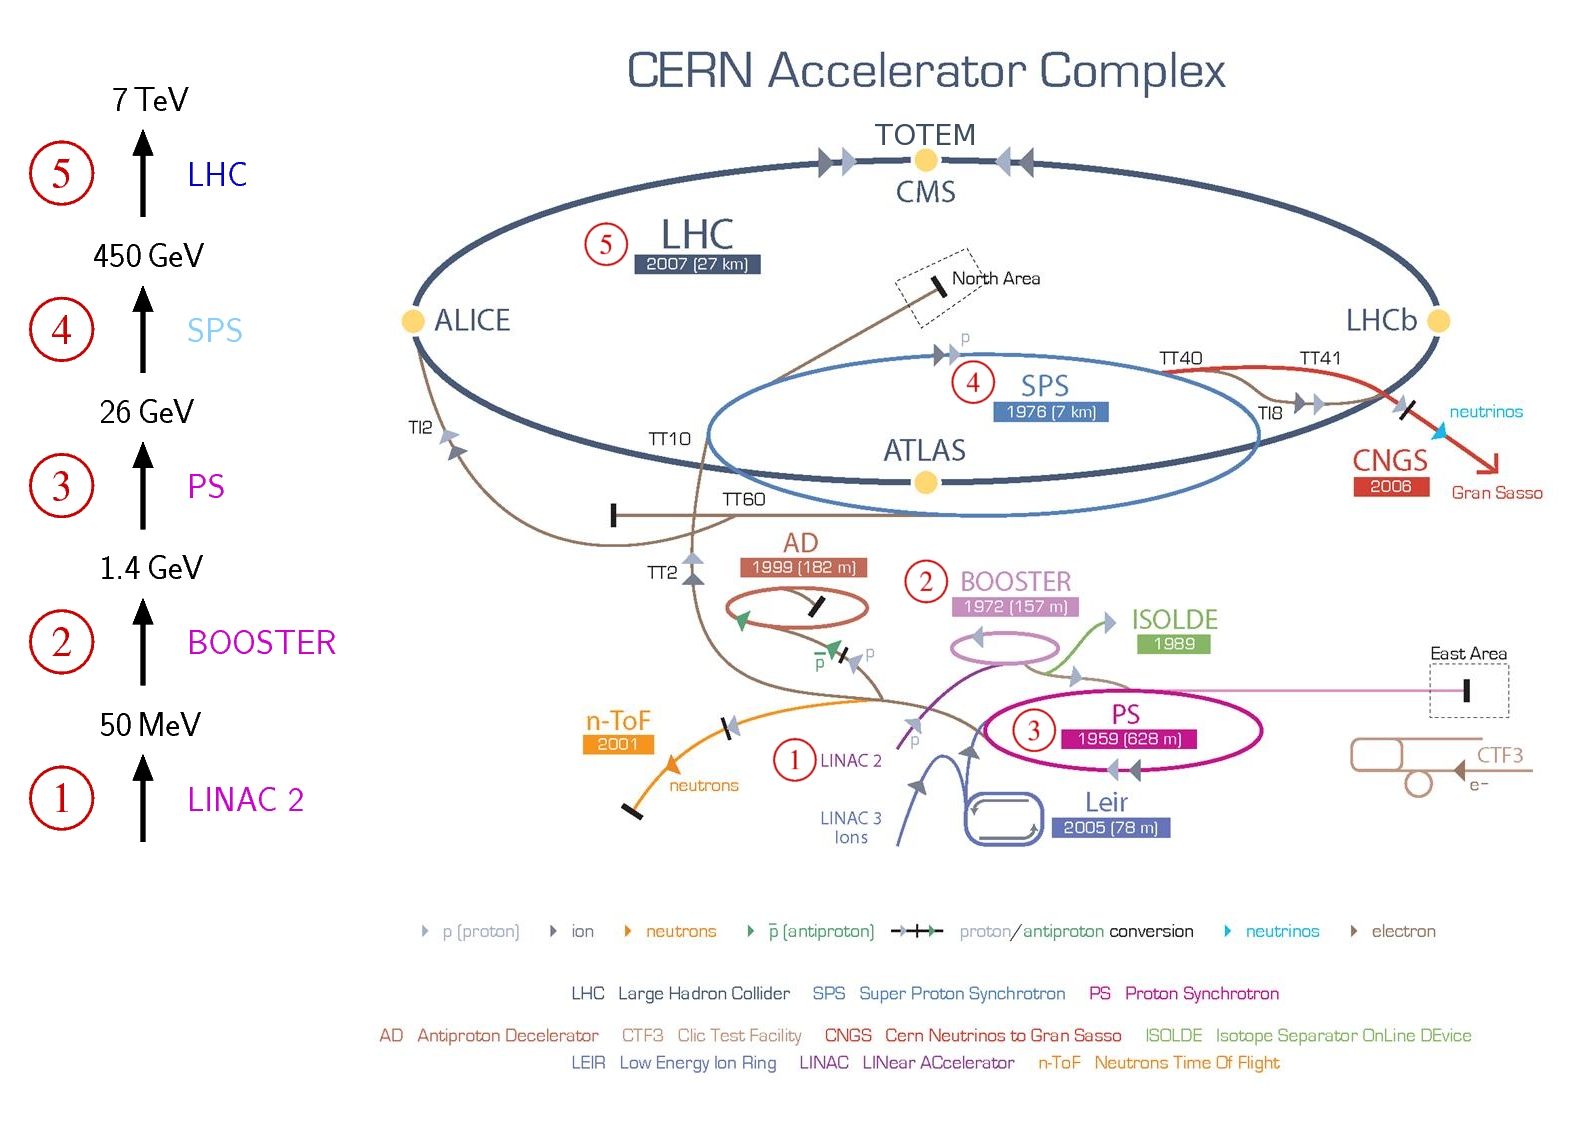
\includegraphics[width=1.0\textwidth]{cms_and_lhc/plots/lhc_complex.png}
     \caption{
Diagram of the LHC accelerator complex showing the five accelerators used to accelerate
protons to their design collision energy of 7\TeV. For the LHC Run II, the highest energy 
achieved for protons is 6.5\TeV.
     }
     \label{fig:lhc_complex}
\end{figure*}



\subsection{LHC Basics}
The LHC accelerator complex has been built up over the years as technology progressed,
physics goals advanced, and continued funding allowed for the expansion and repurposing
of previous accelerators. The LHC acceleration injector chain begins with the LINAC2 linear
accelerator which accelerates protons from rest to an energy of 50 \MeV, 
or $\frac{1}{3}$ the speed of light (c).
The proton acceleration chain begins with a bottle of hydrogen gas which feeds hydrogen
into the source chamber of the LINAC2. A large electric field is applied in the source
chamber which breaks the electron-proton bonds separating the electrons from the protons.
The positive electric charge of the protons allows them to be accelerated by electric
fields. The LINAC2 and the subsequent circular accelerators all use radio frequency (RF)
cavities to accelerate the protons.
With the electrons removed, a group of protons can begin progressing through the accelerator
chain; each grouping of protons accelerated in the LINAC2 eventually become one of the 
circulating proton bunches used for collisions in the LHC.

The LINAC2 feeds into the Proton Synchrotron Booster circular accelerator boosting
the protons to an energy of 1.4 \GeV, or 91.6\% c., followed by the Proton Synchrotron further
accelerating the protons to 26 \GeV, 99.9\% c. The next stage is the Super Proton Synchrotron
accelerating the protons to 450 \GeV, the input energy for the LHC. From 450 \GeV the LHC 
will accelerate the proton bunches to their maximum energy of 6.5 \TeV before 
collisions~\cite{Voss:2009zz}.
A diagram of the LHC accelerator complex can be seen in Figure~\ref{fig:lhc_complex}.



\subsection{LHC Magnets}
The path of the proton and proton bunches is controlled by magnetic fields throughout
the accelerator chain. In all of the circular accelerators, magnetic fields are applied
at right angles to the protons direction of travel which applies a force orthogonal to
the magnetic field and proton velocity bending the proton into a circular path. The LHC
relies on 1232 15-m long superconducting dipole magnets, see Figure~\ref{fig:lhc_dipole},
to bend the path of the protons into a circular path.
The maximum magnetic field the superconducting dipole magnets can attain is 8.33 T which
corresponds to proton beam energy of 7 \TeV. However, the field is limited to 6.5 \TeV by the LHC
beam losses which heat up the interior of the superconducting dipole magnets~\cite{Voss:2009zz}.
The LHC dipole magnets must be cooled by liquid helium to 1.9 Kelvin to maintain their superconducting
characteristics~\cite{lhc_magnets}. The superconducting coils are made from NbTi Rutherford
cables~\cite{1018583}.

\begin{figure*}[htbp]
\centering
     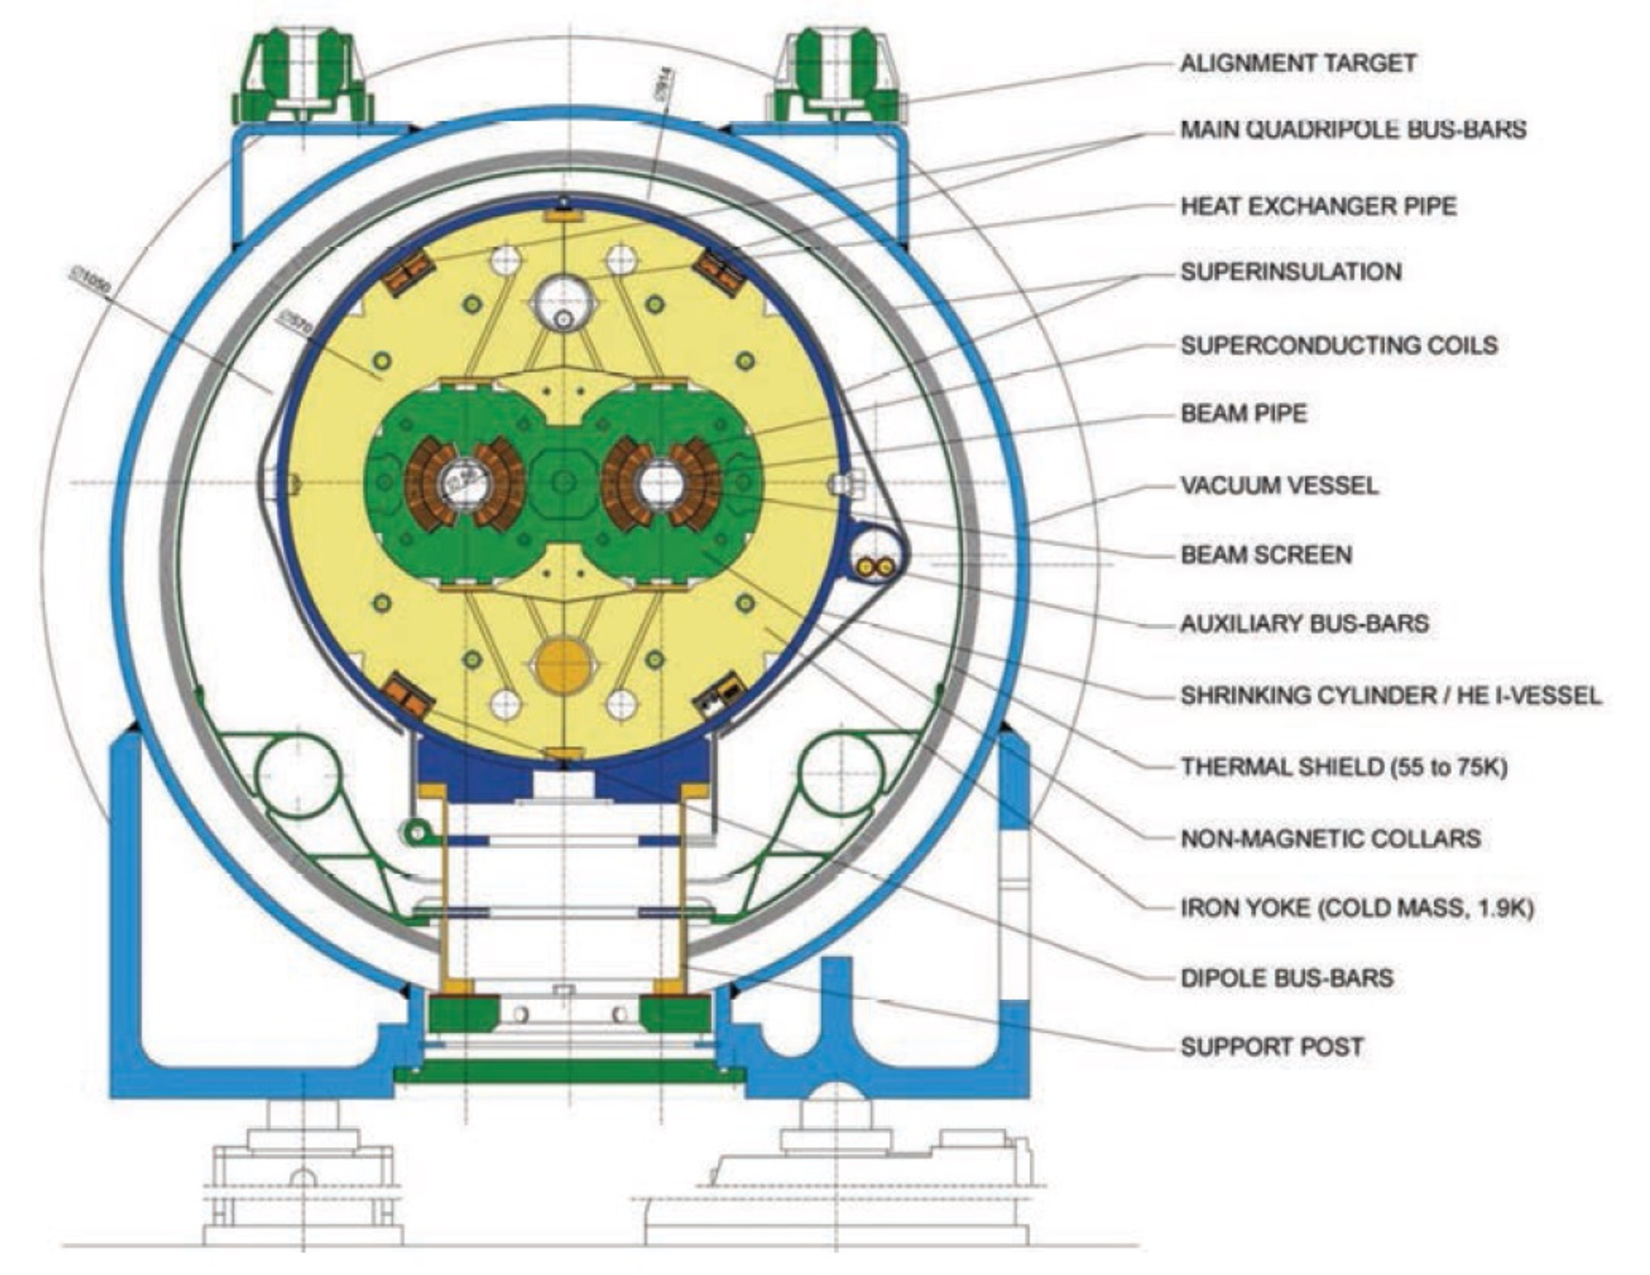
\includegraphics[width=0.6\textwidth]{cms_and_lhc/plots/lhc_dipole_cross_section.pdf}
     \caption{
Cross section of an LHC superconducting dipole magnet showing the two beam pipes in the middle
surrounded by the the superconducting coils.
     }
     \label{fig:lhc_dipole}
\end{figure*}

The LHC superconducting dipole magnets are complimented by 392 main superconducting quadrupole
magnets, 688 sextupole magnets, and 168 octupole-type magnets, which are dedicated to proton 
beam focusing~\cite{lhc_magnets, Voss:2009zz}. 

The accelerator chain and sophisticated magnets of the LHC provide a proton beam segmented
into discrete bunches which can be focused, defocused, and otherwise adjusted to adjust
the rate and characteristics of the proton-proton collision delivered at the beam crossing 
regions~\cite{Benedikt:2004wm} delivering collisions to the LHC experiments. Basic proton 
beam design parameters are detailed in Table~\ref{tab:lhc_beam}~\cite{Benedikt:2004wm}.

\begin{table*}[htbp]
\centering
\begin{tabular}{|l|l|l|l|}
\hline
                  & Units     &   LHC Design  &   2016 LHC Operations \\
\hline
Center of Mass Energy & [\TeV] &    14      &       13      \\
Energy per Beam     & [\TeV]  &       7       &       6.5     \\
Peak Luminosity        & [$\textrm{cm}^{-2}\textrm{s}^{-1}$]   & $1 \times 10^{34}$ & $1.53 \times 10^{34}$  \\
Number of Bunches   & N/A  &   2808    &  2208     \\
Bunch Spacing      & [ns]  &       25      & 25        \\
Protons per Bunch   &  N/A     &   $1.15 \times 10^{11}$   & $1.25 \times 10^{11}$      \\
Bunch Length, total (4$\sigma$) & [ns] &    1.0     &   1.0 \\
\hline
\end{tabular}
\caption{
LHC beam characteristics after LHC ramp has increased the energy of the proton beam from
the input 450 \GeV to collision energy. The bunch length is measured in ns which is the
relevant value for determining the frequency of the LHC RF cavities (400 MHz) used
to accelerate the beam; this length roughly corresponds to 1 meter.
}
\label{tab:lhc_beam}
\end{table*}



\section{The CMS Experiment}
\label{sec:cms}

The Compact Muon Solenoid (CMS) detector is located at point 5 along the LHC ring near Cessy, France. It is
one of the two large general purpose physics detectors in operation at the LHC along with ATLAS. The
CMS detector was inspired by decades of previous high energy particle physics detectors and has as its
primary purpose to detect and measure the characteristics of the Standard Model Higgs boson. The 
detector was designed and built targeting high efficiency and energy resolution for specific Higgs 
boson decay modes. The high granularity of the electromagnetic calorimeter and excellent energy
resolution make it perfect for reconstructing photons from $\PH \to \gamma\gamma$ decays. The
strong, 3.8T magnetic field combined with the muon spectrometer provide excellent Higgs boson
mass resolution in the $\PH \to \PZ\PZ \to \Pgm\Pgm\Pgm\Pgm$ decays. The detector is a large
cylinder 15.0m in diameter and 28.7m in length. It has a mass of approximately 14,000,000kg.

The CMS detector is built out of many subdetectors. Progressing radially outwards from the collision point,
there is first the silicon pixel tracker the the silicon strip trigger systems. Next is the 
electromagnetic calorimeter followed by the hadronic calorimeter. These systems are all contained
within the bore of the CMS superconducting magnet. After the the solenoid there are additional subsystems
embedded within the steel flux-return yoke. In the central region of the detector, there is an 
outer portion of the hadronic calorimeter, and lastly, the muon spectrometer. These systems can all be viewed in
Figure~\ref{fig:cms_detector}.

\begin{figure*}[htbp]
\centering
     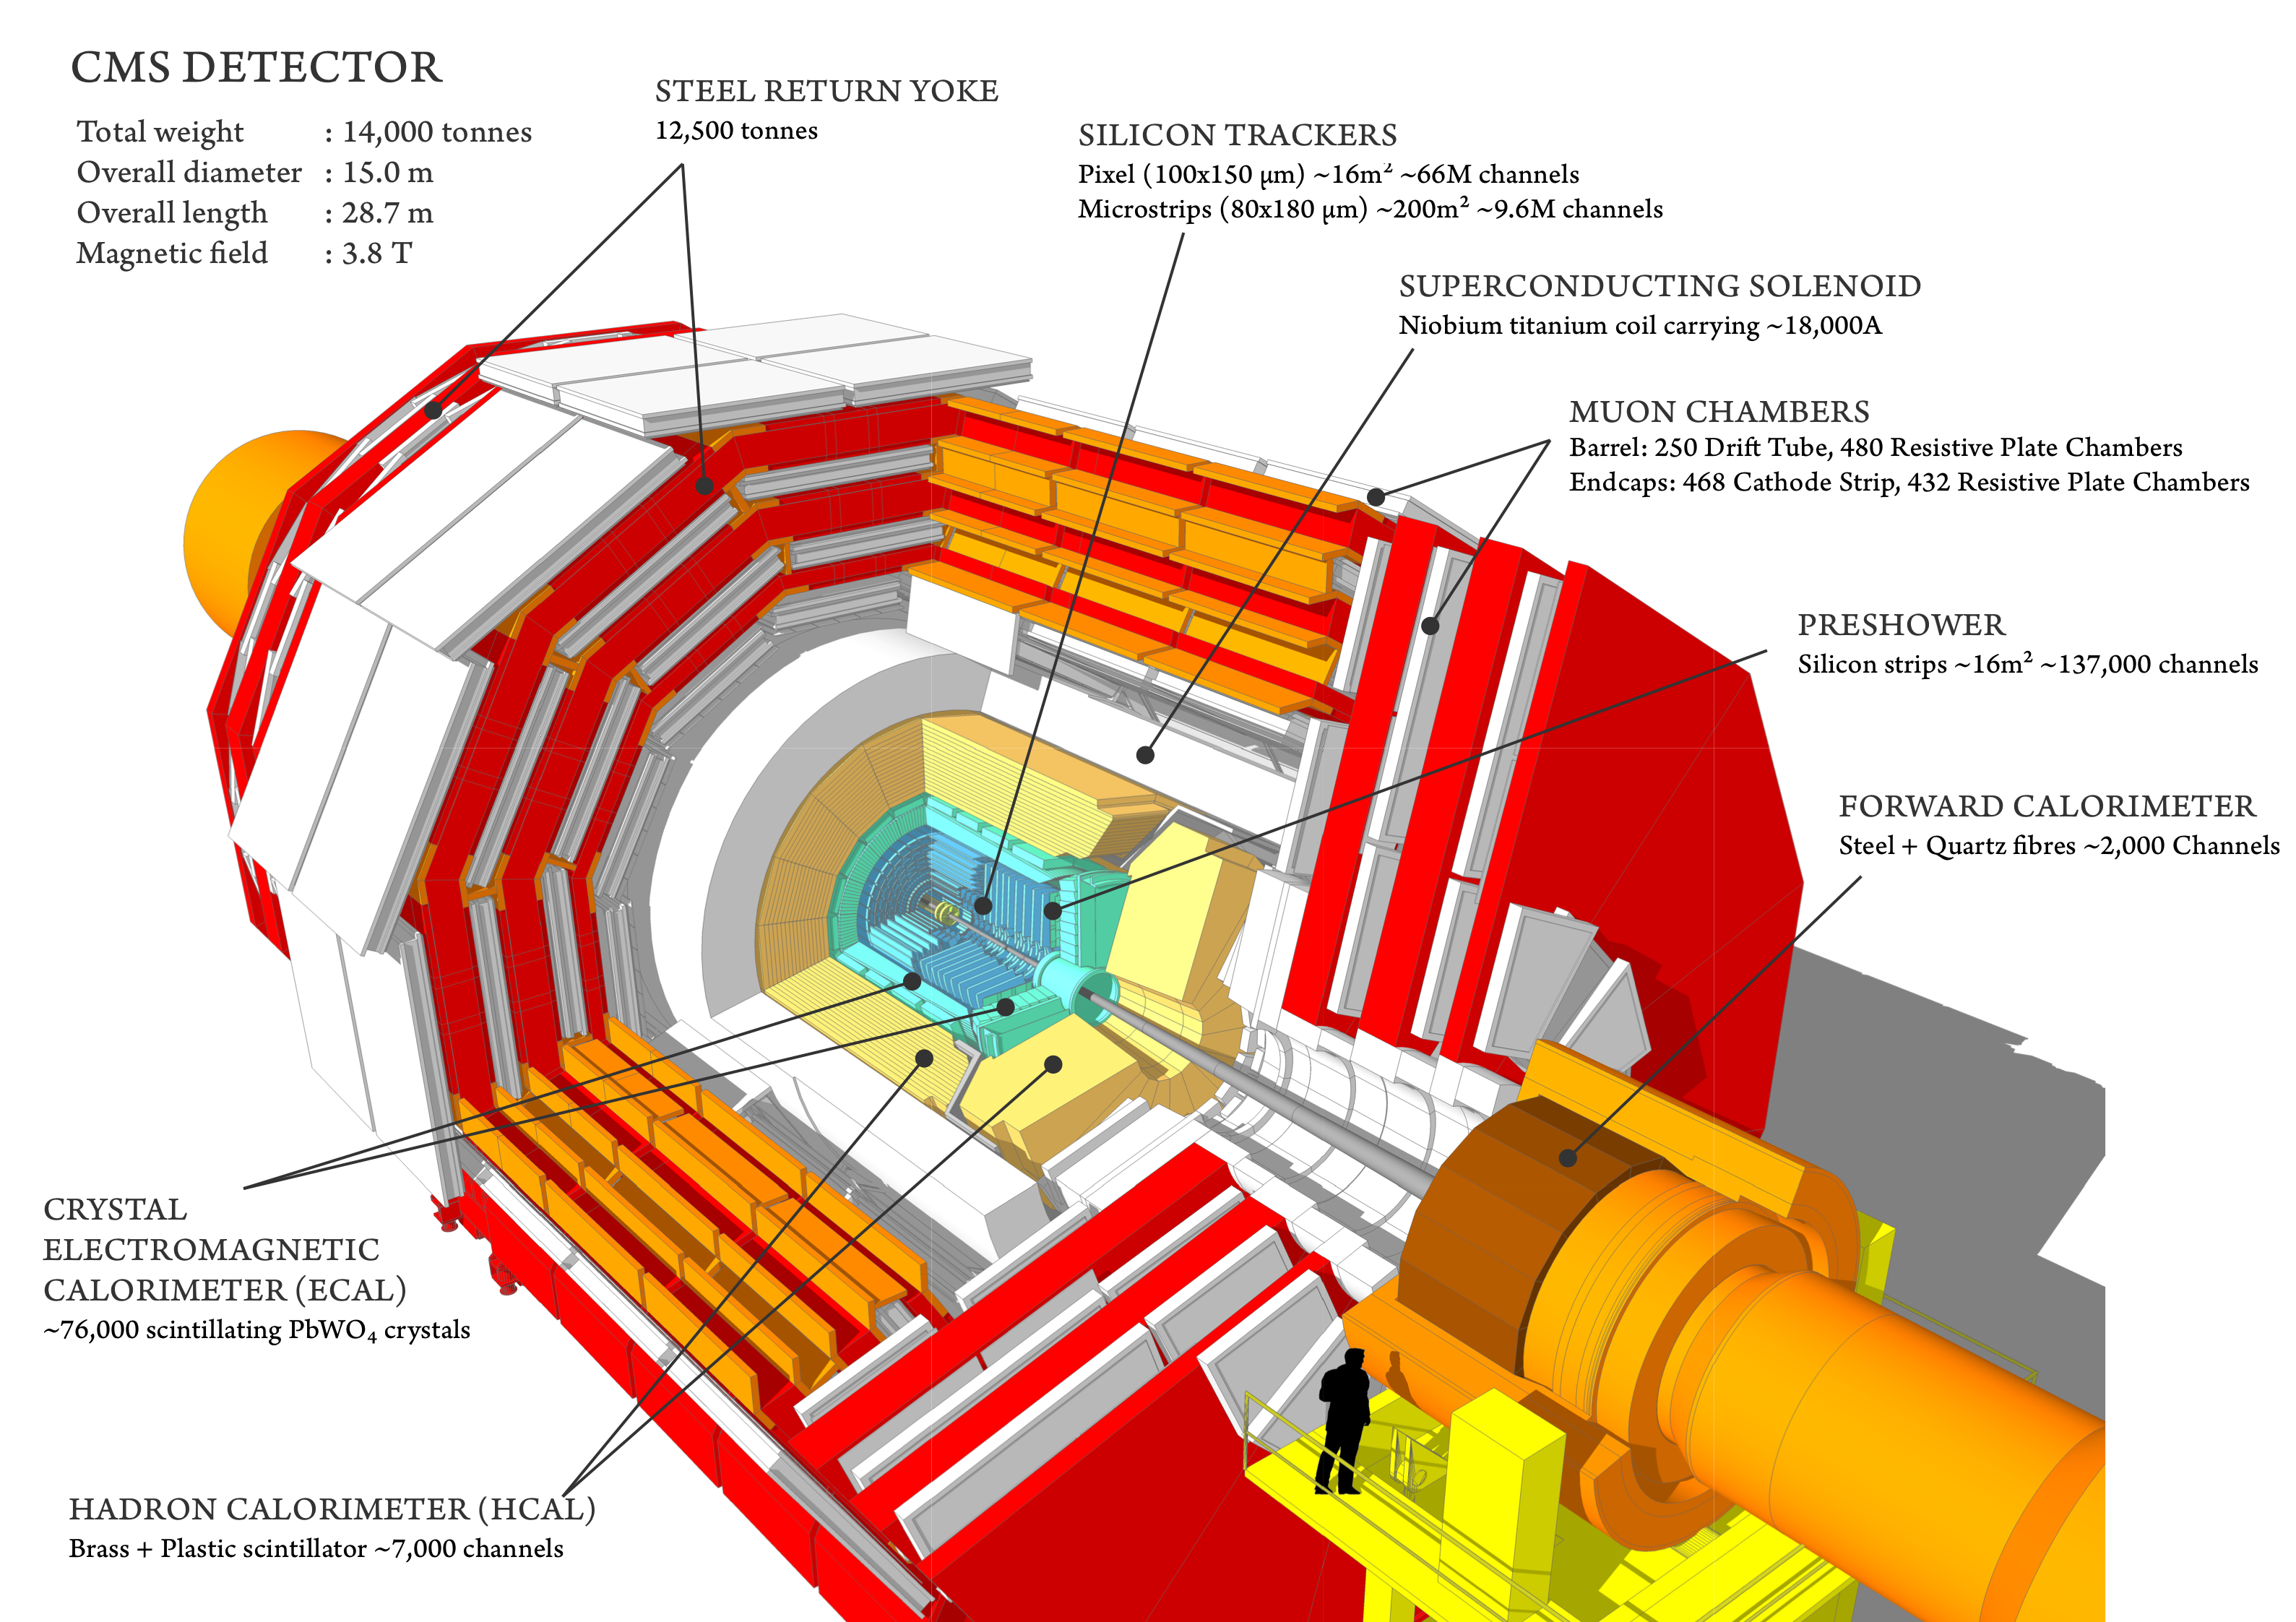
\includegraphics[width=1.0\textwidth]{cms_and_lhc/plots/cms_detector.png}
     \caption{
     }
     \label{fig:cms_detector}
\end{figure*}

Information from the 40 MHz proton-proton collisions is aggregated by a central data acquisition system
and filtered before storage by a two-tiered trigger system~\cite{Khachatryan:2016bia}. 
The first level of the trigger system is composed of custom hardware processors, uses information 
from the calorimeters and muon detectors to select events at a rate of around 100 kHz. The second level of
the trigger, known as the high-level trigger, consists of a farm of commercial processors further
filtering out non-interesting data events resulting in a final event rate of about 1 kHz which is stored
for further processing an analysis.



\subsection{Geometry}
To understand the CMS detector, an understanding of the geometry and coordinate system used by the 
CMS detector is necessary. The CMS detector is a hermetic, cylindrical particle detector surrounding
a central region designed to be the location of the $\pp$ collisions delivered LHC. This middle
point, inside the LHC beam pipe is designated as the origin for the CMS coordinate system, (0,0,0) in
$(x, y, z)$ coordinates. Positive $x$ points towards the center of the LHC ring.
Positive $y$ points vertically upwards. The positive $z$ direction is along the LHC ring in the
clockwise direction when viewed from above. These $(x, y, z)$ coordinates are commonly transformed
into quasicylindrical coordinates when referring to particles, $(\pt, \eta, \phi)$. For a particle,
$\pt$ is:

\begin{equation}
\pt \equiv \sqrt{p^{2}_{x} + p^{2}_{y}}
\end{equation}

$\eta$ is defined using $\theta$ from traditionally spherical coordinates.

\begin{equation}
\eta \equiv -ln\bigg[\tan\bigg(\frac{\theta}{2}\bigg)\bigg]
\end{equation}

$\phi$ is defined in the $x-y$ plane.



\subsection{Superconducting Magnet}
The CMS superconducting magnet, as is noted in the collaboration name, is one of the most fundamental
pieces of the CMS experiment. The superconducting magnet bends the trajectories of charged particles
within the CMS detector. The curve in the flight path of a charged particle can be used to help
calculate the energy or momentum of the particle in accordance with the Lorenetz force.
Within the CMS detector, where the electric field is negligible compared to the magnetic field
from the superconducting magnet, the Lorentz force can be written as~\ref{eqn:lorentz}

\begin{equation}
\textbf{F} = q\textbf{v} \times \textbf{B}
\label{eqn:lorentz}
\end{equation}

relating the mass, acceleration and momentum of a particle with the magnetic field.

The CMS superconducting magnetic is constructed from a 4-layer winding of stabilized
reinforced NbTi conductor. When in operation, the magnet is kept in a superconducting state
by cooling it with liquid helium to a temperature of 4.6 Kelvin. With a nominal current
of 19.14 kA the superconducting solenoid magnet is able to produce a roughly uniform
magnetic field of 3.8 T within its central bore. The magnetic field created is roughly
100,000 times stronger than the Earth's magnetic field. Stronger the magnetic fields produce
more highly curved particle trajectories leading to better momentum and energy measurements.
The central bore is only 6.3 m in diameter
leaving limited room for the CMS tracker and calorimeter systems.



\subsection{Inner Tracking System}
The inner tracking system is composted of two subdetectors, the pixel tracker and the
strips tracker. They are designed to deliver precise and efficient measurement of
the trajectories of charged particles propagating outwards from the LHC delivered
$\pp$ collisions. The tracking systems can be used to reconstruct the origins of
the tracks to reconstruct collision points and secondary decay vertices. The
tracking systems surround the interaction point and have a length of 5.8 m and 
diameter of 2.5 m. Both the pixel and strip trackers have cylindrical barrel
layers and disk-like endcap layers. A schematic of the track systems
can be seen in Figure~\ref{fig:cms_tracker}.

The pixel tracker has three barrel layers at radii between 4.4 cm and 10.2 cm. The
close proximity to the interaction point is helpful for track seeding and vertex
reconstruction discussed in the track reconstruction section~\ref{sec:pf_tracks}.
The silicon strip tracker is composed of 10 barrel detection layers extending 
outwards to a radius of 1.1 m. During the 2016-2017 extended year end technical stop,
the pixel tracker was upgraded to have a fourth detection layer. As 2017 data is not used
in the analyses presented here, details of this upgrade are omitted.
The endcaps of the pixel tracker consist of 2 disks which extend the $\eta$ 
range of the detector to $\abs\eta < 2.5$. The same $\eta$ range is covered in the
strips tracker with 12 disks on each side of the barrel.

\begin{figure*}[htbp]
\centering
     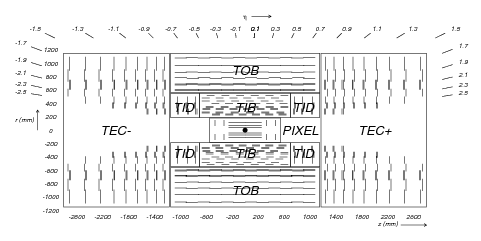
\includegraphics[width=0.8\textwidth]{cms_and_lhc/plots/cms_tracker.png}
     \caption{
Schematic cross section through the CMS tracker. Each line represents a detector module. 
Double lines indicate back-to-back modules which deliver stereo hits.
     }
     \label{fig:cms_tracker}
\end{figure*}

The pixel tracker contains about 66 million individual pixels. The strips tracker
contains 9.3 million individual strips. This phenomenal resolution is necessary
because of the extremely high particle flux through the tracker. During 2016 data
taking, it is estimated that there were $\mathcal{O}( 1000 )$ particles 
traversing the tracker from the more than 20 overlapping simultaneous proton-proton 
interactions during a single bunch crossing. The tracker measures the $\pt$ of 
charged hadrons in the barrel region with a resolution of 1\% for $\pt < 20\GeV$.
The information from the tracker systems is
not used by the L1 trigger. However, the tracker information is heavily used by the HLT to
reduce the event rate from the L1 trigger, 100 kHz, to the final rate of 1000 Hz.

A serious concern during the design of the tracker systems was the amount of
material necessary to build the systems. All of the electronics, hardware, 
cooling systems and wiring contribute to the tracker material budget. Any and all material
located between the interaction region and the calorimeters will reduce the precision 
of the calorimeter energy measurements as well as potentially degrade the track-based
measurement of the energy of a particle. This is because of potential electromagnetic
and/or nuclear interactions between the particle and the tracker material. Figure~\ref{fig:cms_tracker_thickness}
shows the material budget in terms of interaction lengths and radiation lengths as a function
of $\eta$ for the tracker systems.

\begin{figure*}[htbp]
\centering
     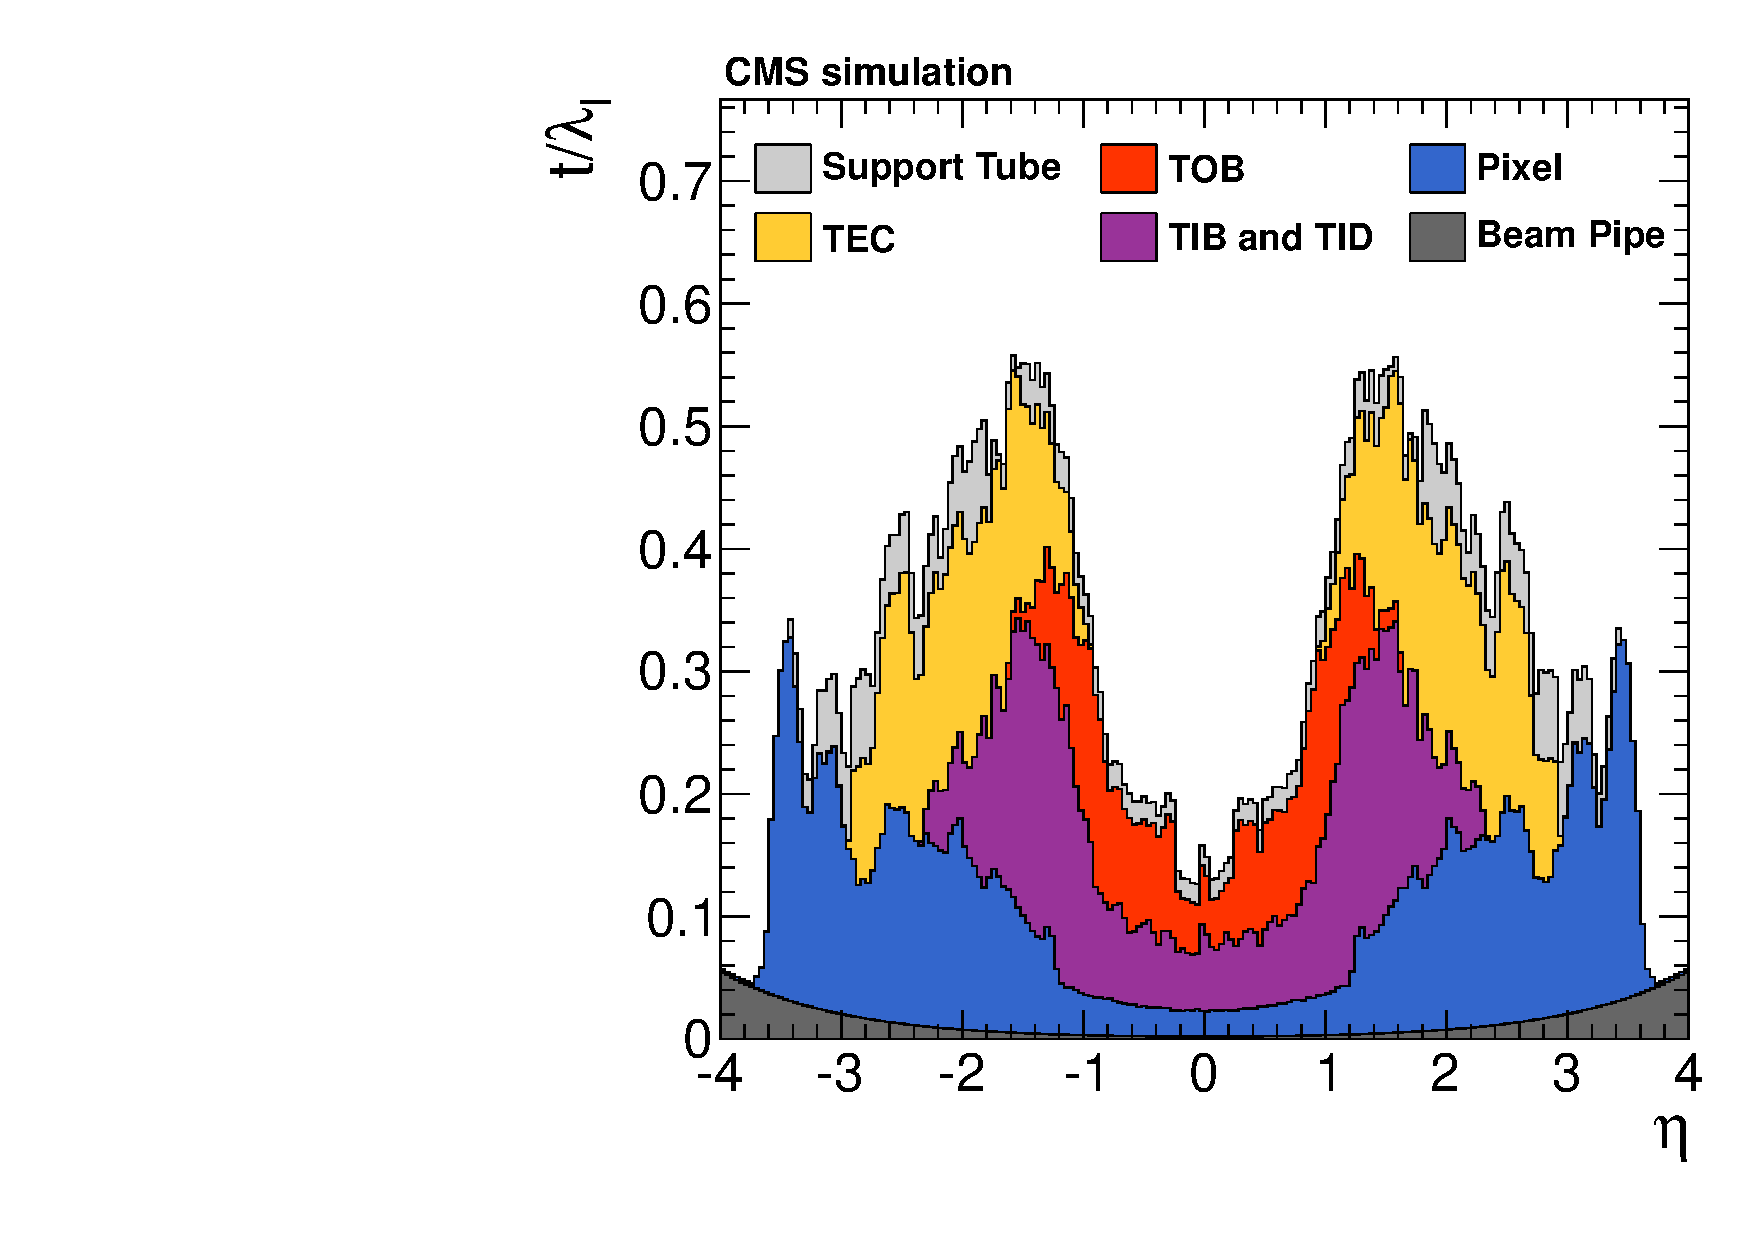
\includegraphics[width=0.4\textwidth]{cms_and_lhc/plots/cms_tracker_thickness_radiationL.pdf}
     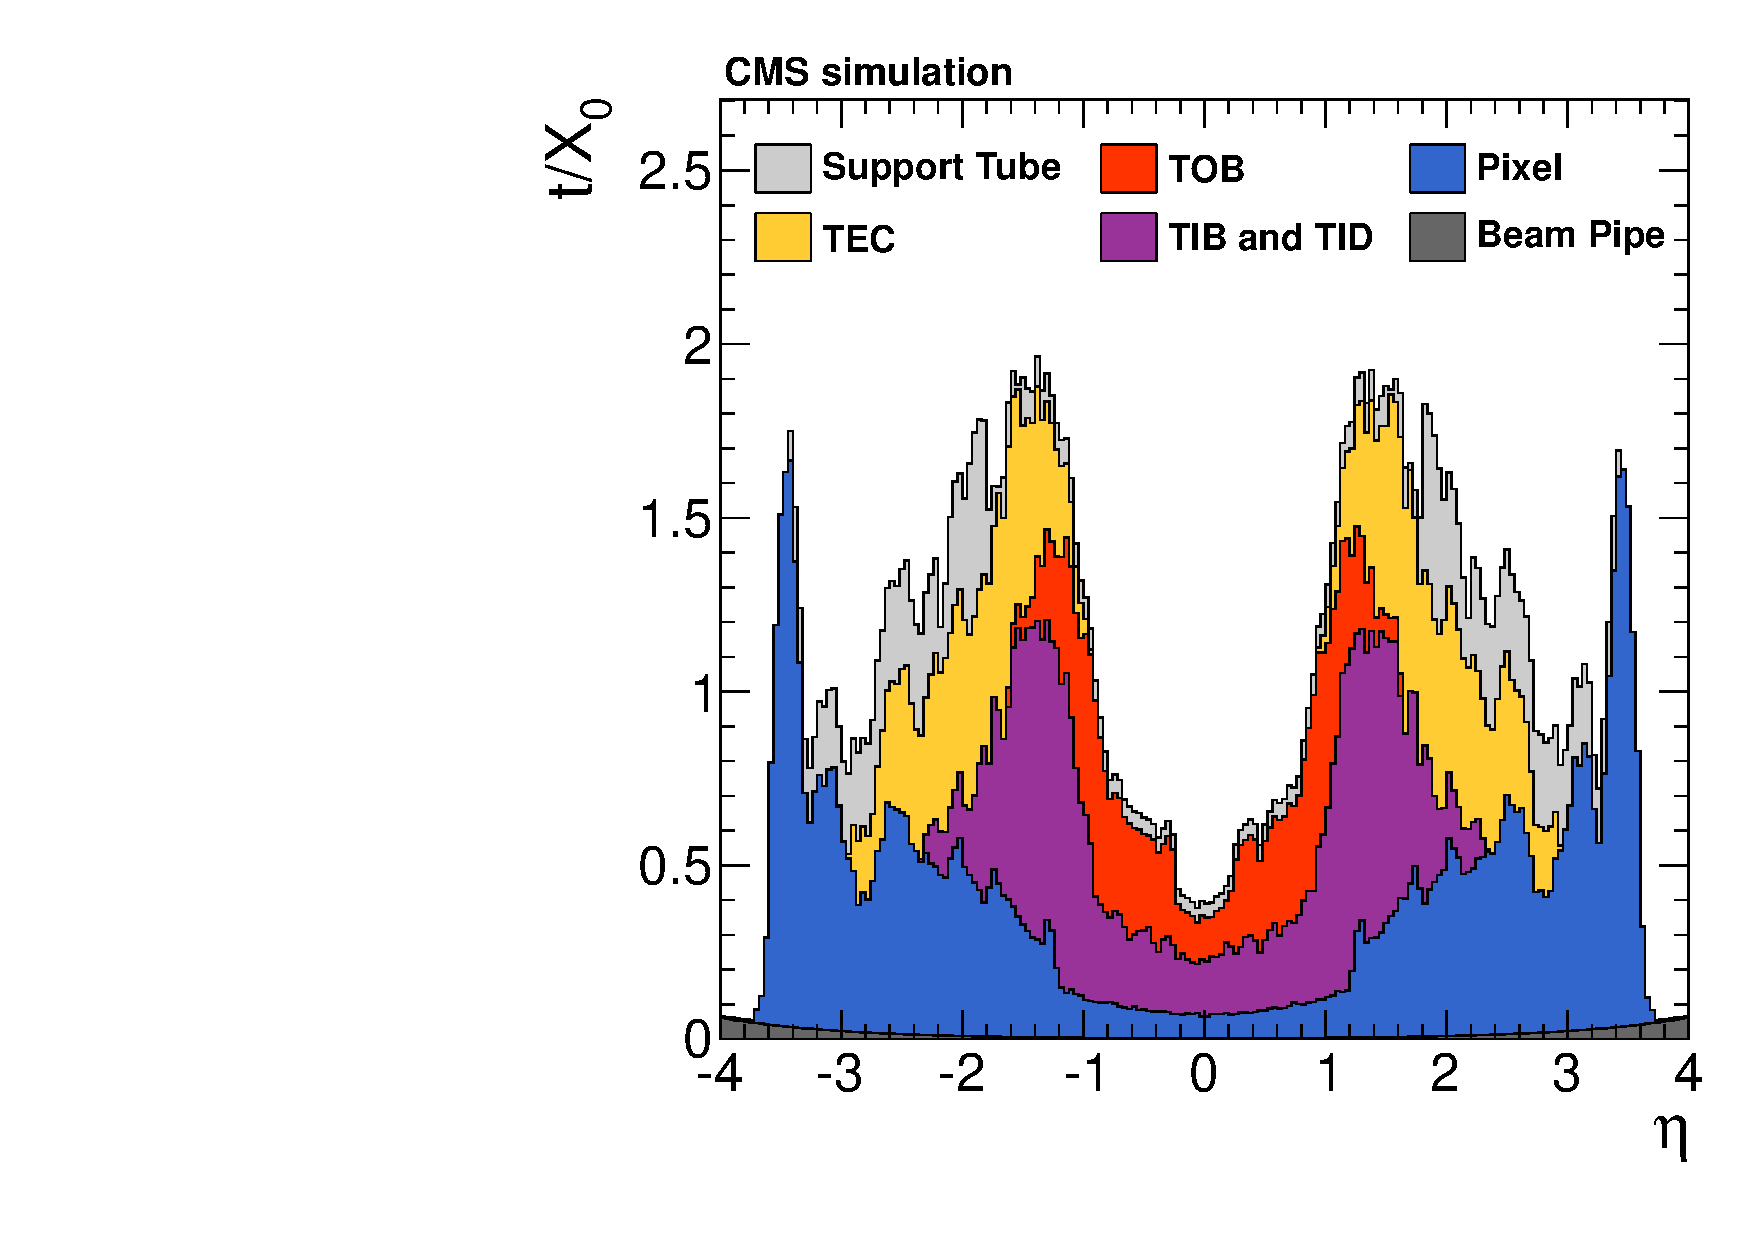
\includegraphics[width=0.4\textwidth]{cms_and_lhc/plots/cms_tracker_thickness_interactionL.pdf}
     \caption{
Total thickness $t$ of the inner tracker material expressed in units of interaction lengths 
$\lambda_{l}$ (left) and radiation lengths $X_{0}$ (right), as a function of the pseudorapidity $\eta$.
     }
     \label{fig:cms_tracker_thickness}
\end{figure*}



\subsection{Electromagnetic Calorimeter}
The electromagnetic calorimeter (ECAL) is a homogeneous calorimeter made of lead 
tungstate $(\textrm{PbWO}_{4})$ crystals. There are 61200 individual crystals mounted
in the barrel region with 360 crystals completing a ring in $\phi$ and 170 crystals
spanning the barrel $\eta$ range, $\abs\eta < 1.479$. 
The ECAL endcap detectors cover the $\eta$ range $1.479 < \abs\eta < 3.0$. The multiple
ECAL systems can be seen in Figure~\ref{fig:cms_ecal}.
The ECAL barrel crystal cross-section is approximately $0.0174 \times 0.0174$ 
in \etaphi, or about $22 \times 22 \textrm{mm}^{2}$
on the front face of a crystal. Twenty-two millimeters is also the Moli\`ere radius
for $(\textrm{PbWO}_{4})$, meaning, on average, an electromagnetic shower could be
contained by 4 crystals. As mentioned earlier, this fine grain resolution is extremely
helpful for precise energy measurements of electrons and photons and specifically
enables the $\PH \to \gamma\gamma$ analysis to resolve a relatively narrow Higgs
boson mass peak. 

The ECAL barrel crystals are 230 mm in length corresponding to a
radiation length of 25.8 $X_{0}$ which is sufficient to contain 98\% of the energy
of electrons and photons up to 1\TeV. Despite the large number of radiation lengths,
the crystals have an interaction length, $\lambda_{l}$, of about 1.0. This causes
roughly two thirds of the hadrons passing through the ECAL to start showering
within the ECAL. 

As particles interact with the crystals, energy is deposited at a rate of about 4.5
photoelectrons per \MeV~\cite{dafinei_auffray_lecoq_schneegans_1994}.
The scintillation decay time of the $(\textrm{PbWO}_{4})$ crystals is approximately the
same order of magnitude as the LHC bunch crossing time; about 80\% of the light is emitted in 25 ns.
This provides the fast response necessary to separate out-of-time energy ECAL deposit
from a given LHC bunch crossing. To read-out the energy deposited in each barrel
crystal, there is an avalanche photodiode (APD) mounted to the backside-facing surface
of the crystal. For the endcap crystals, a more radiation hardened readout is used,
vacuum phototriodes (VPTs). typical ECAL electronics noise 
$\sigma ^{\text{ECAL}} _{\text{noise}}$ is measured to be $\approx$ 40 (150) \MeV 
per crystal in noise the barrel (endcaps).
The energy resolution of the ECAL barrel crystals is given by
Equation~\ref{eqn:ecal_res}.

\begin{equation}
\label{eqn:ecal_res}
\frac{\sigma}{E} = \frac{2.8\%}{\sqrt{E/\GeV}} \oplus \frac{12\%}{E/\GeV} \oplus 0.3\%
\end{equation}



\begin{figure*}[htbp]
\centering
     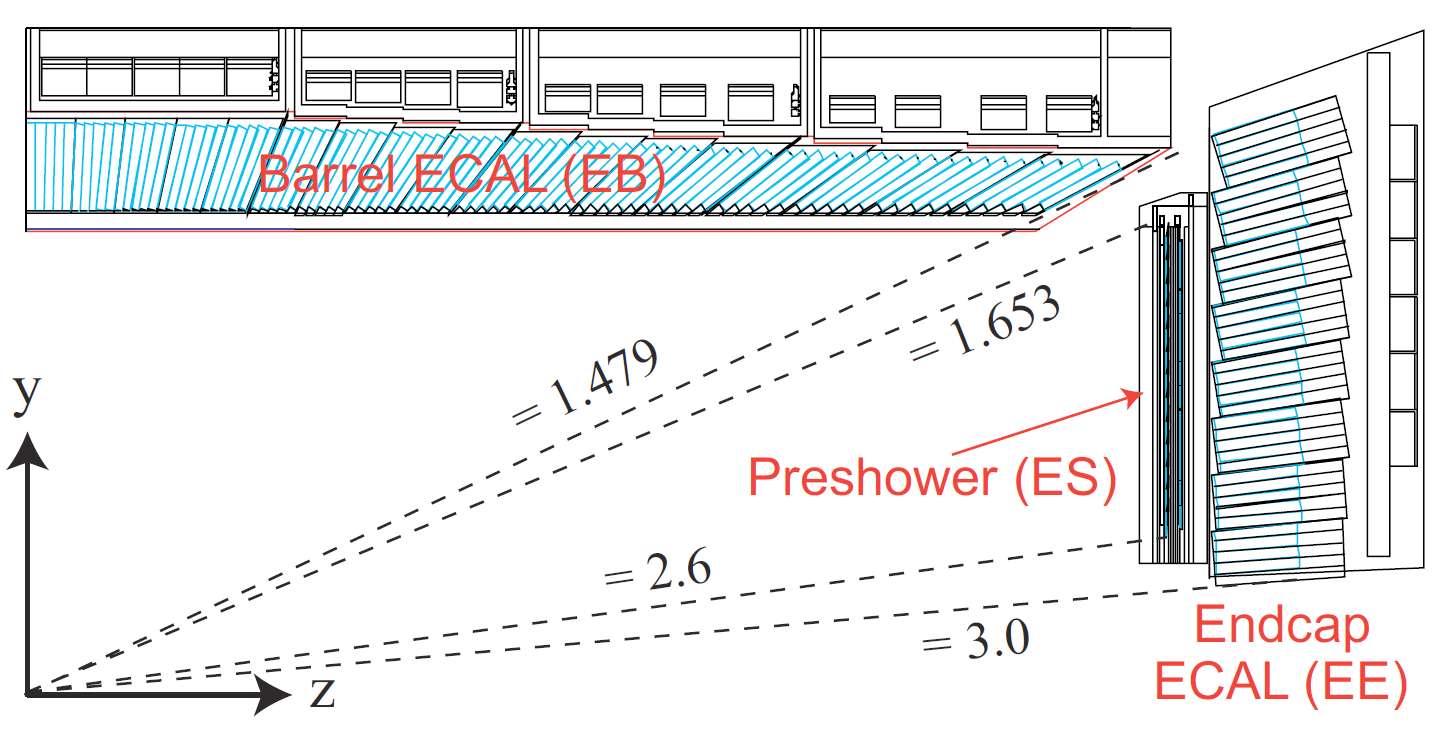
\includegraphics[width=0.8\textwidth]{cms_and_lhc/plots/cms_ecal.png}
     \caption{
Longitudinal view of the CMS detector depicting the ECAL subdetector.
The crystals are inclined towards the interaction region.
     }
     \label{fig:cms_ecal}
\end{figure*}



\subsection{Hadronic Calorimeter}
The hadronic calorimeter(s) (HCAL) provide the necessary energy measurements
to reconstruct charged and neutral hadrons in CMS. These particle are the
primary measurable constituents in ``jets'' and hadronically decay $\tau$
leptons. Additionally, measurement of the energy imbalance from a collision
can indicate the presence of neutrinos or possibly exotic particles~\cite{CMS-Proposal}.
The HCAL is segmented into four calorimeters: the barrel detector, the endcap detector,
the forward hadronic detector, and the barrel outer detector. 
The barrel detector is a sampling calorimeter covering $\abs\eta < 1.3$. It is built
from flat brass absorber plates interleaved with plastic scintillator segments to
measure and readout the deposited energy. The HCAL barrel has coarser granularity
than the ECAL; each segment is $0.087 \times 0.087$ in \etaphi which covers the
same area as 25 ECAL crystals.

The HCAL barrel occupies the space between the ECAL and the superconducting magnet
from a radial distance of 1.77 m to 2.95 m form the beam line. Particle propagating
outwards at an angle of $\eta = 0$ will encounter the thinnest portion of the
HCAL barrel corresponding to 5.82$\lambda_{l}$. The effective thickness increases
with $\eta$ resulting in 10.6$\lambda_{l}$ at $\abs\eta = 1.3$. The HCAL detector
is depicted in Figure~\ref{fig:cms_hcal}.

To increase the effective
thickness in the barrel region, $\abs\eta < 1.3$, an outer hadronic calorimeter is placed 
outside the superconducting magnet which complements the barrel calorimeter
extending the effective thickness to a minimum of 11.8$\lambda_{l}$ in the barrel. 
The HCAL endcap system partially overlaps with the barrel detector and ranges from
$1.3 < \abs\eta < 3.0$.

Beyond $\abs\eta = 3$, the forward hadronic calorimeter, located
11.2 m from the interaction point, extend the $\eta$ coverage out to $\abs\eta = 5.2$.
On average, 760\GeV per proton-proton interaction is deposited into the forward 
calorimeters, compared to only 100\GeV for the rest of the detector~\cite{Chatrchyan:2008zzk}.
At higher $\abs\eta$ values, closer to the beam pipe, 
The high particle and radiation flux, at high $\abs\eta$ values, close to the beam pipe,
severely limits the types of detector systems which can survive years of LHC operating
conditions. Because of this, the forward hadronic calorimeter is not the same style sampling
calorimeter like the rest of HCAL. Instead it uses Cherenkov-based, 
radiation-hard, fused-silica quartz fibers embedded in grooves within the steel structure
of the absorber material.

The energy resolution of the HCAL barrel has been measured using test beams~\cite{Elvira:800406}, and is:
\begin{equation}
\label{eqn:hcal_res}
\frac{\sigma}{E} = \frac{115\%}{\sqrt{E/\GeV}} \oplus 5.5\%
\end{equation}
For the forward HCAL system the energy resolution is~\cite{Baiatian:951395},
\begin{equation}
\label{eqn:hcal_res}
\frac{\sigma}{E} = \frac{280\%}{\sqrt{E/\GeV}} \oplus 11\%
\end{equation}
These two equations show the much poorer energy resolution of HCAL compared to ECAL.
There are multiple reasons for this include the fact that the HCAL is a sampling 
calorimeter thus much of the energy deposits occur in absorber layers and the 
size of the deposits must be estimated and calibrated for.
Typical HCAL electronics noise $\sigma ^{\text{HCAL}} _{\text{noise}}$ 
is measured to be $\approx$ 200 MeV per tower about 5 times the noise level of
the ECAL barrel crystals, but comparable to the ECAL endcap crystals.

\begin{figure*}[htbp]
\centering
     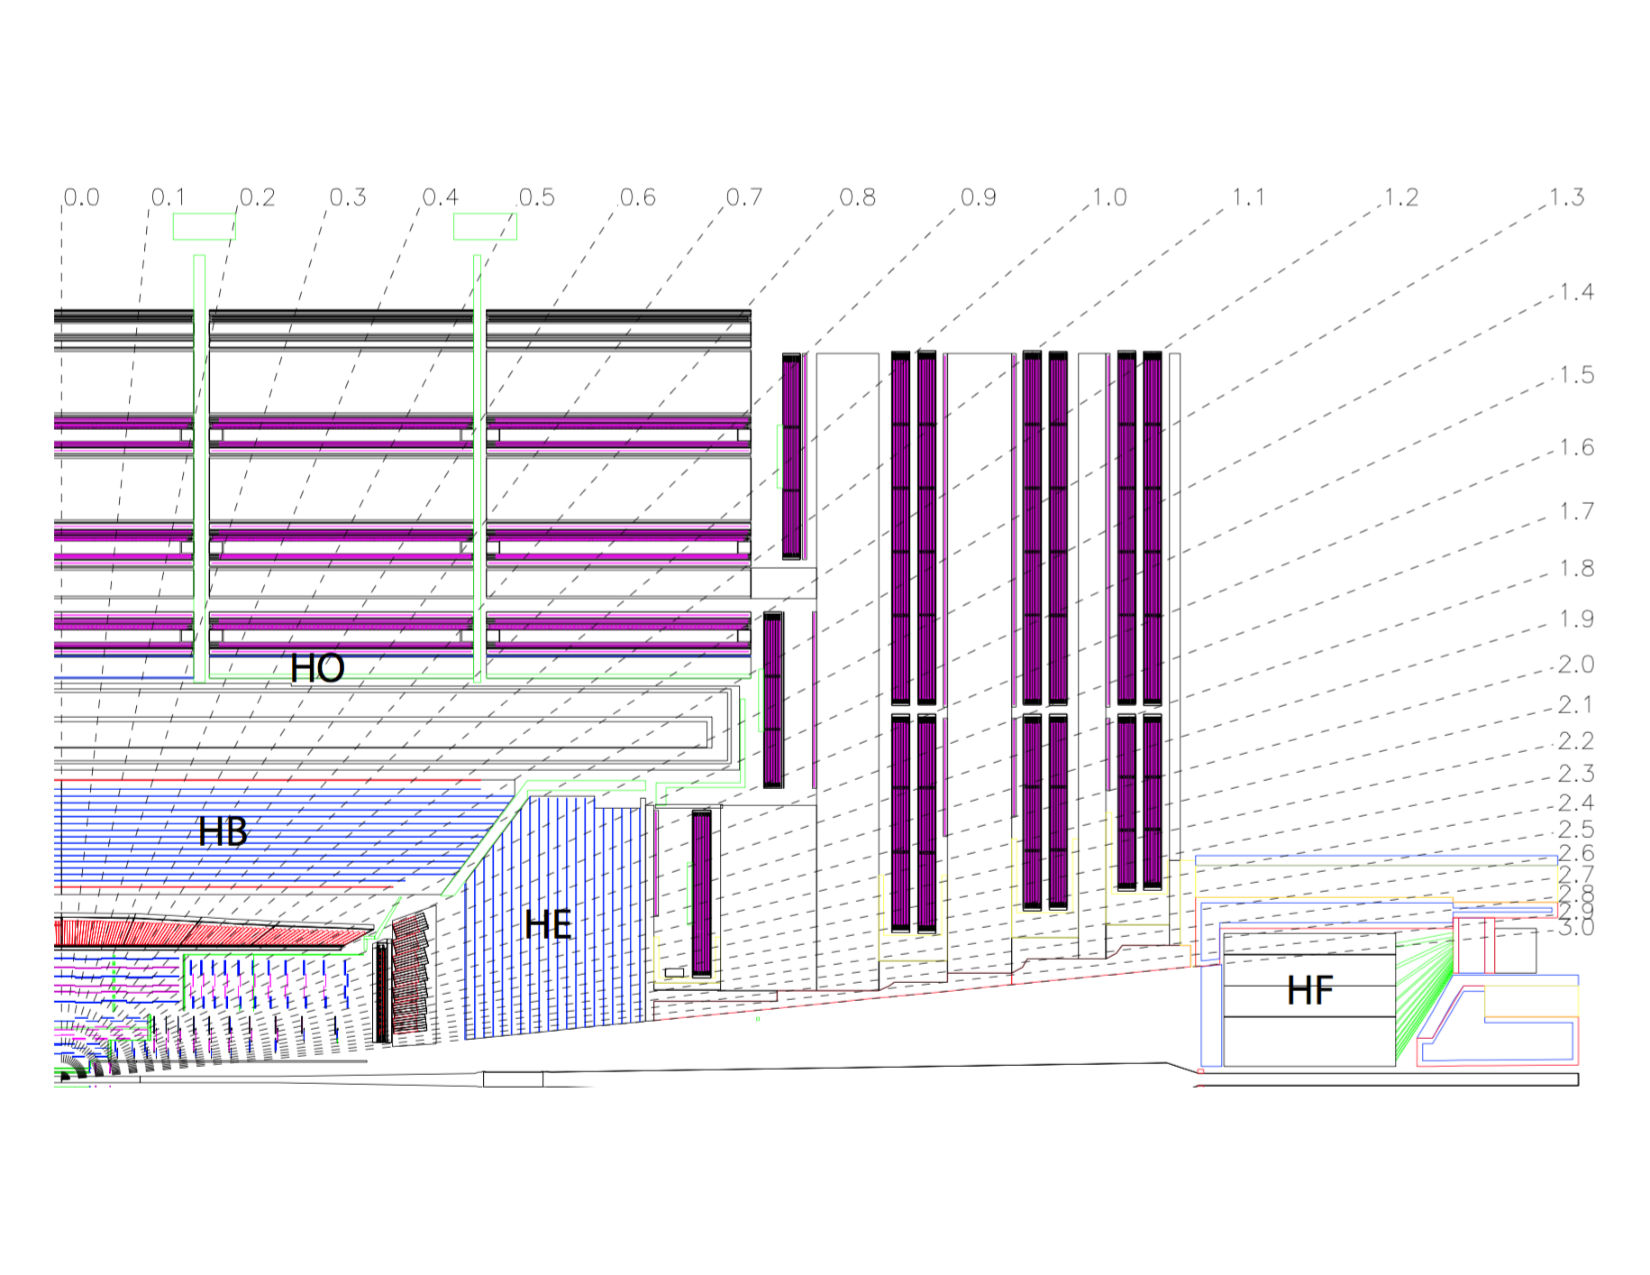
\includegraphics[width=0.8\textwidth]{cms_and_lhc/plots/cms_hcal.pdf}
     \caption{
Longitudinal view of the CMS detector showing the locations of the hadron 
barrel (HB), endcap (HE), outer (HO) and forward (HF) calorimeters. The
effective thickness of the HB detector increases with increasing $\abs\eta$.
     }
     \label{fig:cms_hcal}
\end{figure*}




\subsection{Muon System}
With ``Muon'' in the name of the experiment, it is clear that the muon spectrometer
is important to the physics goals of the CMS experiment. Excellent muon reconstruction, 
identification, and momentum measurement allows Higgs analyses, such as $\PH \to \PZ\PZ$
where $\PZ\PZ \to \Pgm\Pgm\Pgm\Pgm$ to achieve their most precise mass measurements. Using
2016 data, the $\PH \to \PZ\PZ$ analysis measured the Higgs boson mass with an uncertainty
of approximately 0.2\%, 
$m^{4\Pgm}_{\textrm{H}} = 124.94 \pm 0.25 (\stat) \pm 0.08 (\syst)\GeV$~\cite{cms-2016-hzz}.
In addition to the mentioned functions of the muon system, the high purity of reconstructed
muons makes the system very useful for selecting data events to store.
The muon spectrometer is composed of three subsystems, the drift tubes (DT) which cover
$\abs\eta < 1.2$, the cathode strip chambers (CSC) which cover $0.9 < \abs\eta < 2.4$, and
the resistive plate chambers (RPC) covering $\abs\eta < 1.6$, see Figure~\ref{fig:cms_muon_syst}.

\begin{figure*}[htbp]
\centering
     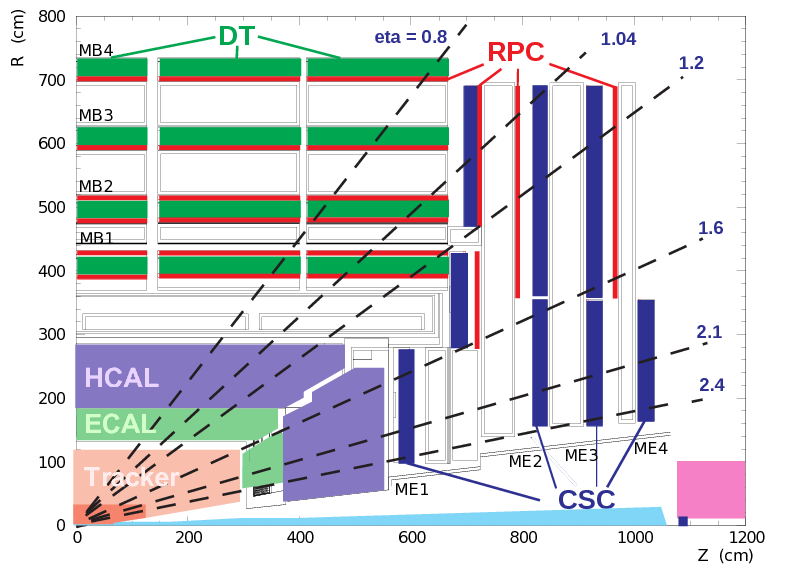
\includegraphics[width=0.8\textwidth]{cms_and_lhc/plots/cms_muon_syst.png}
     \caption{
Layout of one quadrant of CMS. The four DT stations in the barrel (MB1-MB4, green), the four CSC stations in the endcap (ME1-ME4, blue), and the RPC stations (red) are shown.
     }
     \label{fig:cms_muon_syst}
\end{figure*}

The muon subsystems are each embedded within the magnet's flux-return yoke. Each system
detects particles through gas ionization techniques. 
When passing through ionizing gas detectors, charged particles leave a trail of ionized gas 
molecules which can be detected and measured by different techniques.

The drift tubes are used in the barrel region
because of the low expected particle rate and the relatively low strength of the local
magnetic field (which is well contained in the flux-return yoke through the barrel region).
The DTs rely on 172,000 2.4 m long sensitive wires maintained at a high voltage to detect the traces
of passing charged particles. The wires are housed in a drift cell with a maximum path length
and time of drift of 21 mm and 380 ns using a gaseous mixture of 
$85\% \, \textrm{Argon} \, + \, 15\% \, \textrm{CO}_{2}$~\cite{CMS-Proposal}. The drift cell size and drift
time are small enough to avoid high occupancy levels during collisions data taking.
A detailed schematic of a DT cross-section is in Figure~\ref{fig:cms_muon_dt}.

\begin{figure*}[htbp]
\centering
     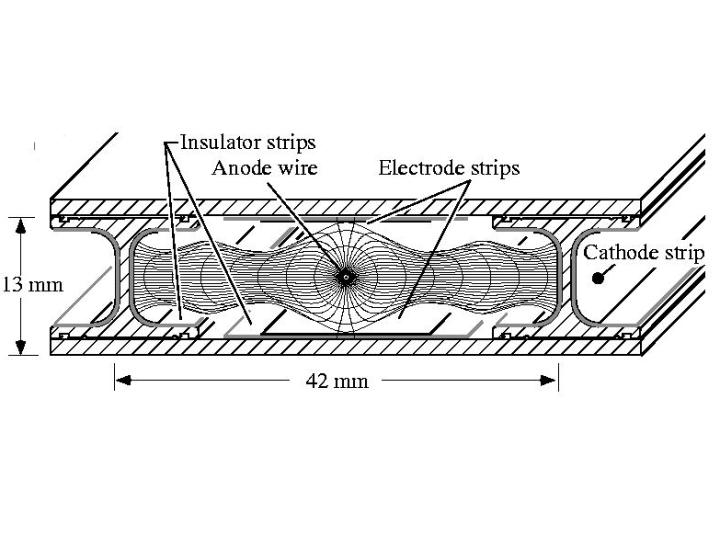
\includegraphics[width=0.7\textwidth]{cms_and_lhc/plots/cms_muon_dt.jpg}
     \caption{
Schematic of a drift tube cell showing drift lines leading to/from the wire 
and isochrones three of which are seen as the concentric lines surrounding the wire. The voltages applied to the 
electrodes are +3600V for wires, +1800V for strips, and −1200V for cathodes.
     }
     \label{fig:cms_muon_dt}
\end{figure*}

Progressing outwards from the barrel region towards higher $\abs\eta$ values, the background 
particle flux increases as does the non-uniformity of the magnetic field in the spacing between
the flux-return yoke. These considerations lead to a different required muon detection technology.
In the two endcap regions of CMS the muon system uses cathode strip chambers arranged as large
disks much like the other subsystem endcaps. The CSCs have a fast 
response time, fine segmentation, and are more radiation resistant than the DTs. The CSC system
is depicted in Figure~\ref{fig:cms_muon_csc} showing the relative arrangement of the anode
wires to the cathode strips. The muon coordinate along the anode wires (the $\phi$ coordinate) 
is obtained by interpolating charges induced on strips~\cite{cms_csc_gas}.
The CSC subsystem has a nominal gas mixture of 
$40\% \, \textrm{Argon} \, + \, 50\% \, \textrm{CO}_{2} \, + \, 10\% \, \textrm{CF}_{4}$.


\begin{figure*}[htbp]
\centering
     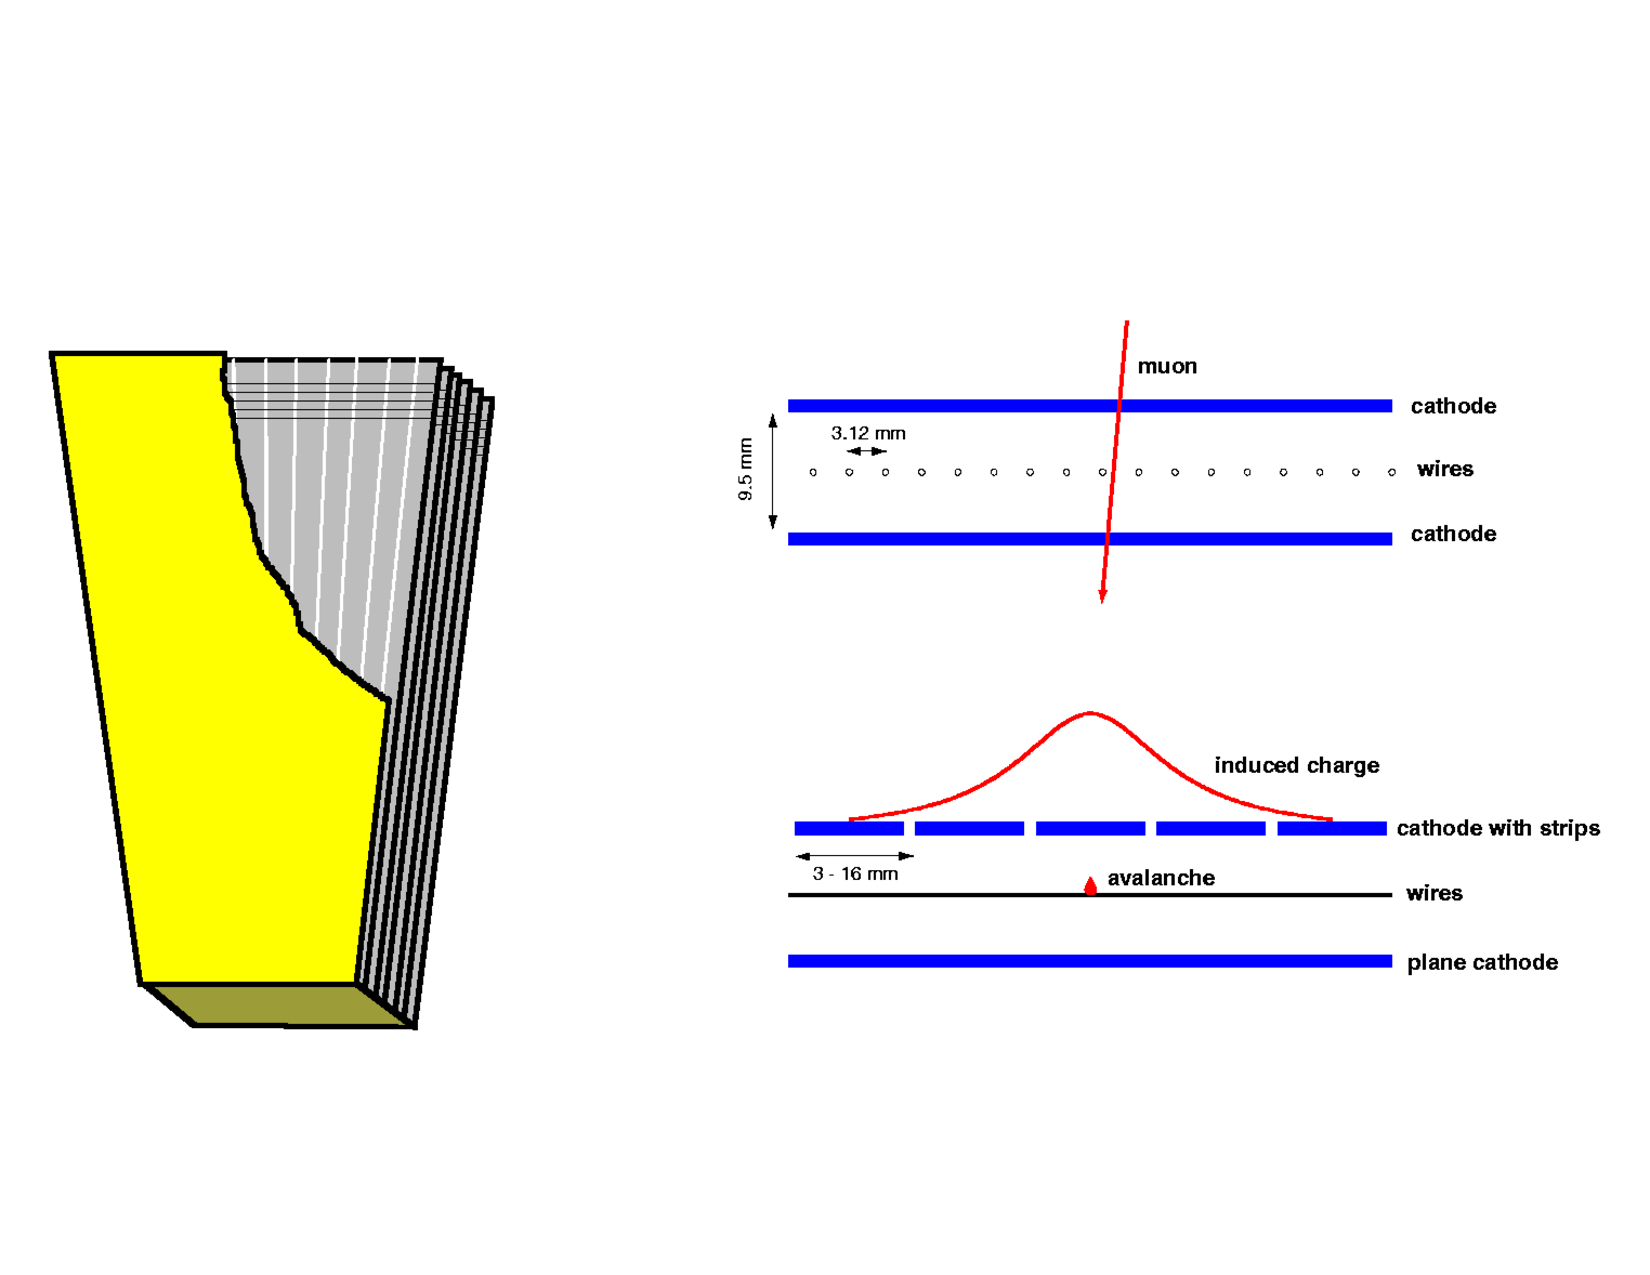
\includegraphics[width=0.8\textwidth]{cms_and_lhc/plots/cms_muon_csc2.pdf}
     \caption{
(left) Schematic of a CSC module composed of 7 trapezoidal panels with 6 gas gaps between
the panels. The cut away of the top panel reveals the anode wires used to 
detect ionized molecules from a passing muon. The anode wires running horizontally and 
the cathode strips running vertically.
(right) Two diagram showing the inner dimensions of a CSC gas gap. The two views
show how the orthogonal configuration of the anode wires and cathode strip can be used
to localize the positions of a transversing muon.
     }
     \label{fig:cms_muon_csc}
\end{figure*}

To increase the timing precision of the muon spectrometer a third subsystem was added
built from resistive plate chambers (RPC) which cover the barrel and a portion of the endcap
region of the detector, $\abs\eta < 1.6$. The RPCs are gaseous parallel-plate ionizing gas 
detectors with two gas chambers per module. The RPC system is used to compliment the excellent spacial resolution of the
DTs and CSCs with a high precision timing measurement that can resolve with which LHC bunch
crossing a certain energy deposit is associated. The timing resolution is comparable
to that of scintillator-based detectors~\cite{rpc_dev}.

The RPCs are constructed with two chambers per module that are both operated in avalanche mode.
Common pick-up read-out strips are located in between the two chambers. With the common
 read-out strips, the total induced signal is the sum total of the signal in each of the
chambers. The two-fold signal allows the RPCs to operate at a lower voltage than a single
chamber detector and leads to increased efficiency. 
The RPC subsystem is operated with a nominal gas mixture of 
$96.2\% \, \textrm{R134a} \, + \, 3.5\% \, i\textrm{C}_{4}\textrm{H}_{10} \, + \, 0.3\% \, \textrm{SF}_{6}$~\cite{CMS-Proposal}.
An example of the
double-chamber construction is in Figure~\ref{fig:cms_muon_rpc}.

\begin{figure*}[htbp]
\centering
     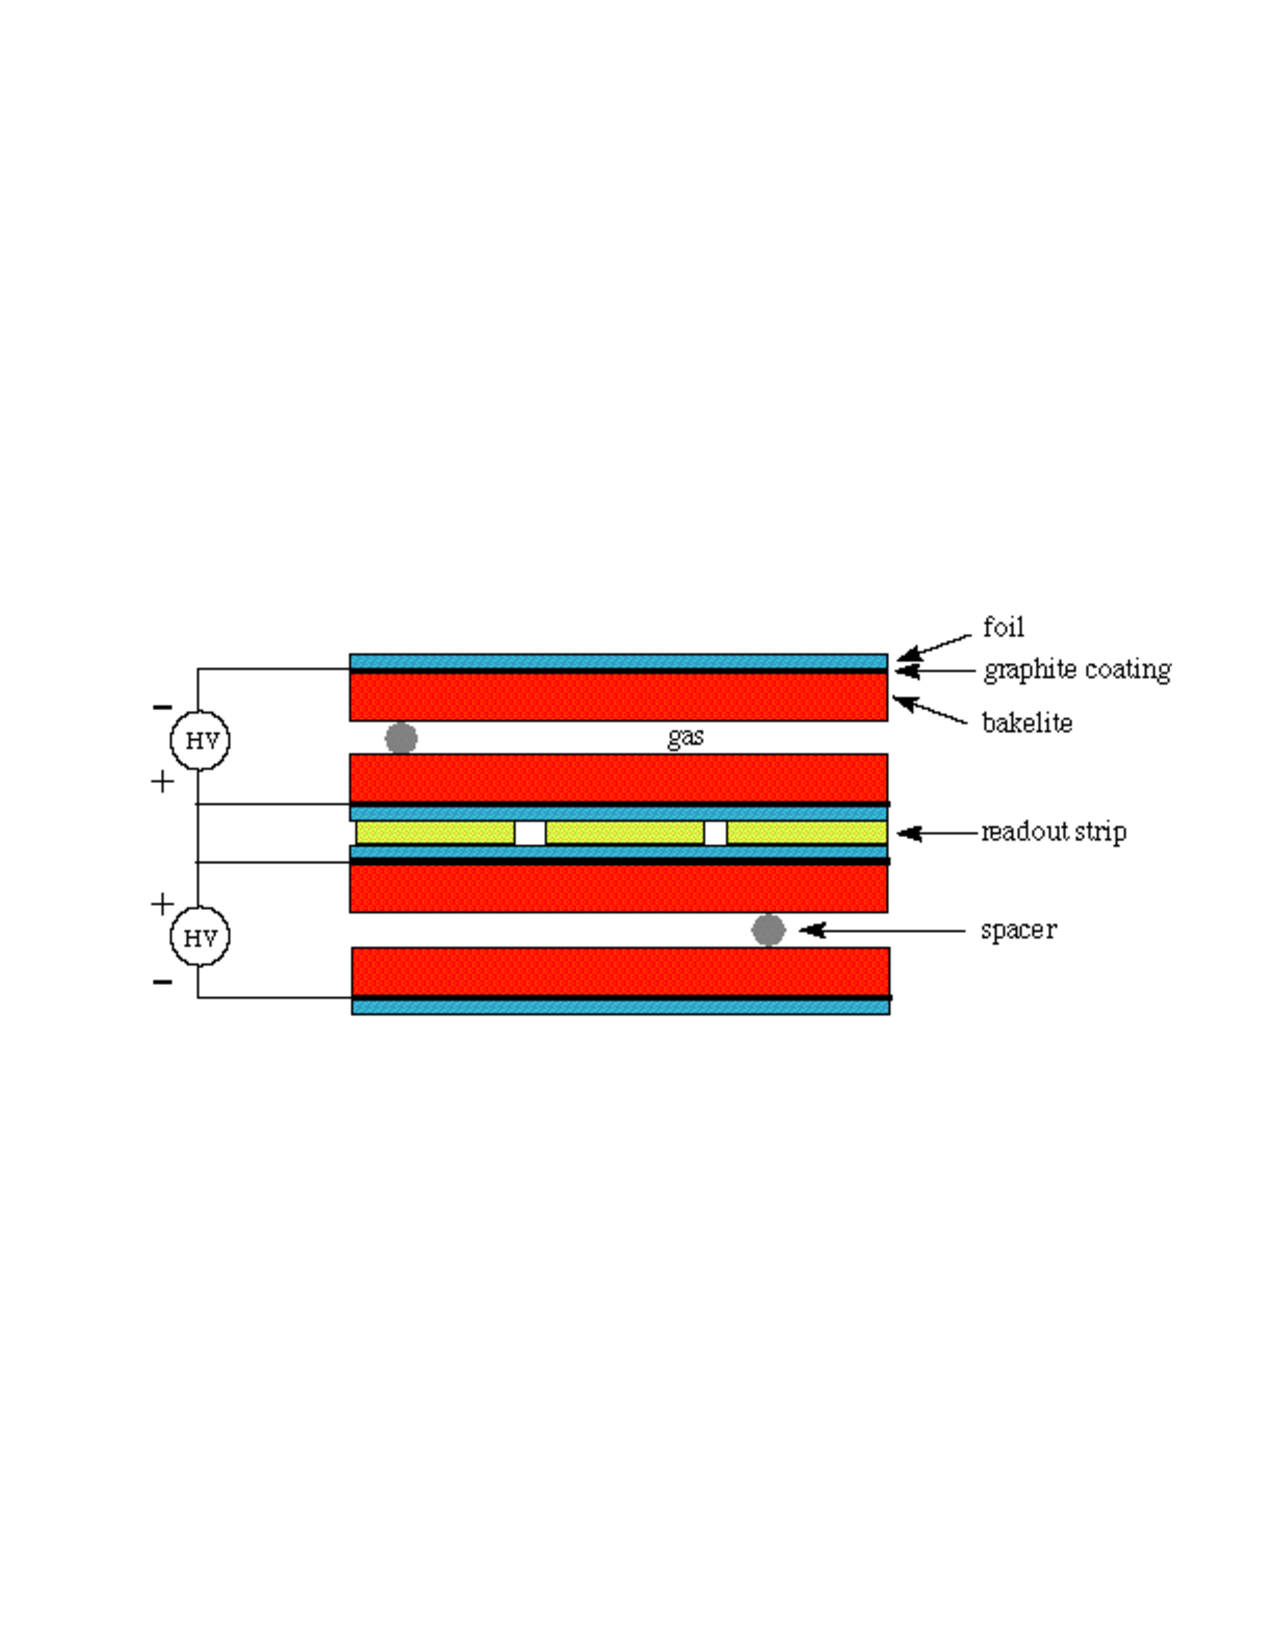
\includegraphics[width=0.6\textwidth]{cms_and_lhc/plots/cms_muon_rpc.pdf}
     \caption{
A sketch of a double-chamber RPC. The gas chamber is 2 mm wide and is surrounded by two
bakelite layers 2 mm thick each.
     }
     \label{fig:cms_muon_rpc}
\end{figure*}



\subsection{Trigger and Data Acquisition}
The CMS Trigger and Data Acquisition (DAQ) system is designed and built to readout detector
information from each of the CMS subdetectors, make a rapid assessment if the the content
associated with a specific LHC bunch crossing is worth storing for future physics analysis,
and, finally, delivering the event content to storage. The 40 MHz bunch crossing rate of
the LHC makes this a remarkable challenge. The Trigger and DAQ system must operate rapidly
and in close synchronization so that the event content read-out by each subdetector is attributed
to the proper LHC bunch crossing. In total, the trigger system reduces the throughput rate from the
initial 40 MHz to a storage rate of roughly 1 kHz. Storing more events for physics analysis is
always desired, but with each event requiring roughly 1 MB of disk space for storage in its
raw format, storing many more events is not currently an option for the CMS experiment based 
on available storage space~\cite{CMS-Proposal}. 



\subsubsection{Level-1 Trigger}
The CMS Trigger system is broken down into two tiers. The two tiered approach relies on
the first level, the Level-1 (L1) Trigger, to assess basic event content from each LHC
bunch crossing and make an initial determination of whether the event appears interesting for
future analysis or not. The L1 Trigger reduces the input 40 MHz rate to a more manageable
100 kHz. The speed and throughput requirements of the L1 Trigger necessitate that the system 
is built from dedicated, custom hardware. The L1 Trigger is restricted to 4 $\mu$s of latency
to make the determination of whether the event should be passed the the next tier or whether
the event should be deleted~\cite{Khachatryan:2016bia}. The latency requirement eliminates
the possibility of using inner tracker information as well as full ECAL crystal-level
granularity.

The L1 Trigger utilizes input from the calorimeter subsystems, ECAL and HCAL, and the muon 
subsystems, DT, CSC, and RPC. A systems flow chart of the L1 Trigger is in
Figure~\ref{fig:cms_l1t}. The L1 Trigger is split into two path the calorimeter system
and the muon system which merge paths at the micro global trigger ($\mu$GT) for the
final L1 Trigger decision. The muon system is composed of three muon triggers which are
geometrically divided by $\abs\eta$. The Barrel Muon Track Finder covers $\abs\eta < 0.85$,
the Overlap Muon Track Finder covers $0.85 < \abs\eta < 1.25$, and the Endcap Muon
Track Finder covering $1.25 < \abs\eta < 2.4$. The resulting track from the three
track finder systems are the L1 muon candidates.

Information from the calorimeter subdetectors is aggregated by the
Calorimeter Layer-1 trigger where initial processing and calibrations are completed.
Each of the 18 Layer-1 cards (CTP7s) receive calorimeter information from a single 20 degree $\phi$ slice 
of the detector~\cite{Cadamuro:2017slr}. The HCAL and ECAL input granularity is $0.087 \times 0.087$ in \etaphi
through the barrel. Above $\abs\eta > 2.1$ the $\eta$ dimension becomes larger with $\phi$
staying constant reflecting the geometry of the ECAL and HCAL systems. In the L1 Trigger, 
ECAL information represents as a trigger tower, the sum of $5 \times 5$ groupings of 
ECAL crystals~\cite{Khachatryan:2016bia}.

Following the 18 Layer-1 CTP7s is the Layer-2 trigger which further aggregates
data from a singular event so that one Layer-2 hardware card (MP7) has calorimeter data for
the full detector. This allows computation
of full event-based characteristics like the missing transverse energy, see 
Section~\ref{sec:obj_reco_met} for a description of missing transverse energy. A detailed
layout of the L1 calorimeter trigger can be found in Figure~\ref{fig:cms_l1t} beginning
with the 18 Layer-1 cards and progressing to the 9 main Layer-2 MP7s plus 3 spares.
The Layer-2 MP7s execute rapid, firmware-based, algorithms to reconstruct basic physics
objet candidates such as electrons and $\gamma$s, hadronically decaying $\tau$ leptons, 
``jets'', and energy sums~\cite{Cadamuro:2017slr}. For a description of ``jets'', 
see Section~\ref{sec:obj_reco_jets}.
The calorimeter-based and muon system-based physics objects are sent to the $\mu$GT
where the final decision is made whether to pass an event along to the HLT or not.

\begin{figure*}[htbp]
\centering
     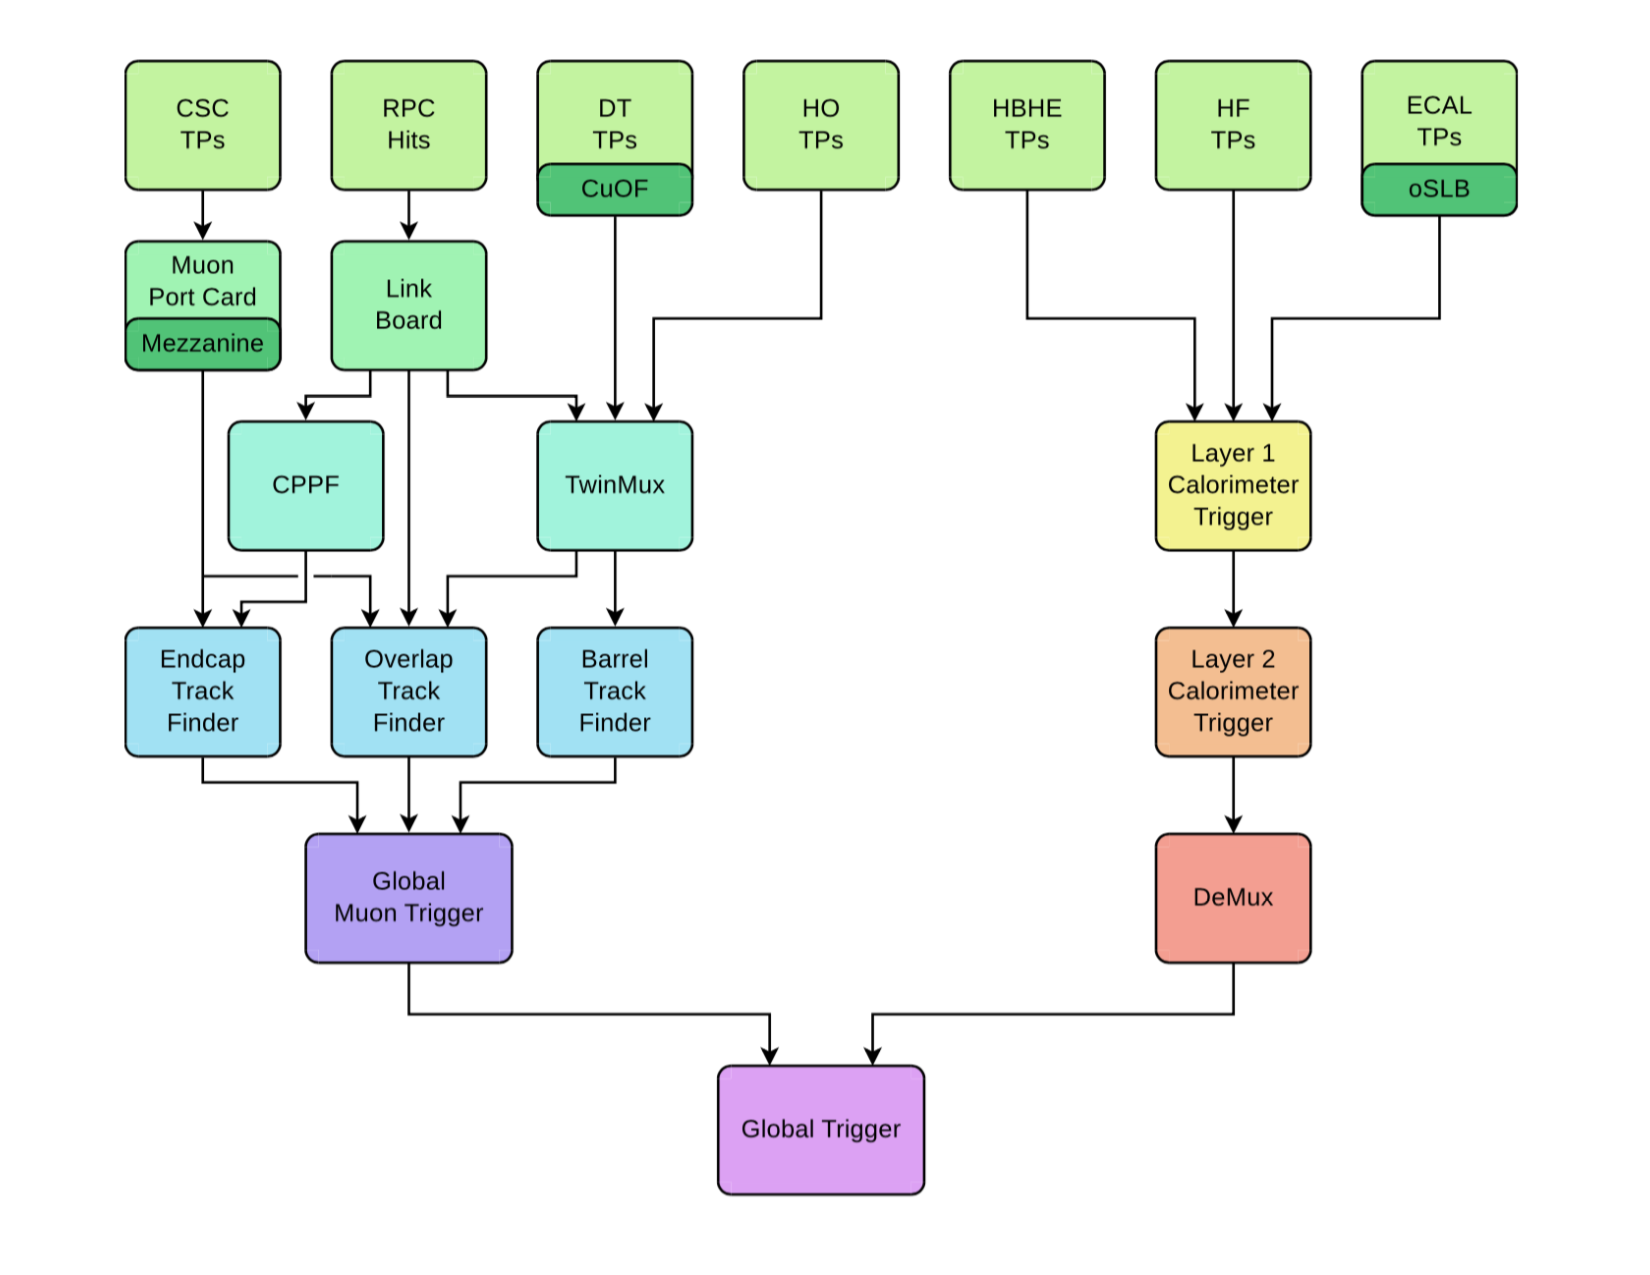
\includegraphics[width=0.49\textwidth]{cms_and_lhc/plots/cms_l1t_system.pdf}
     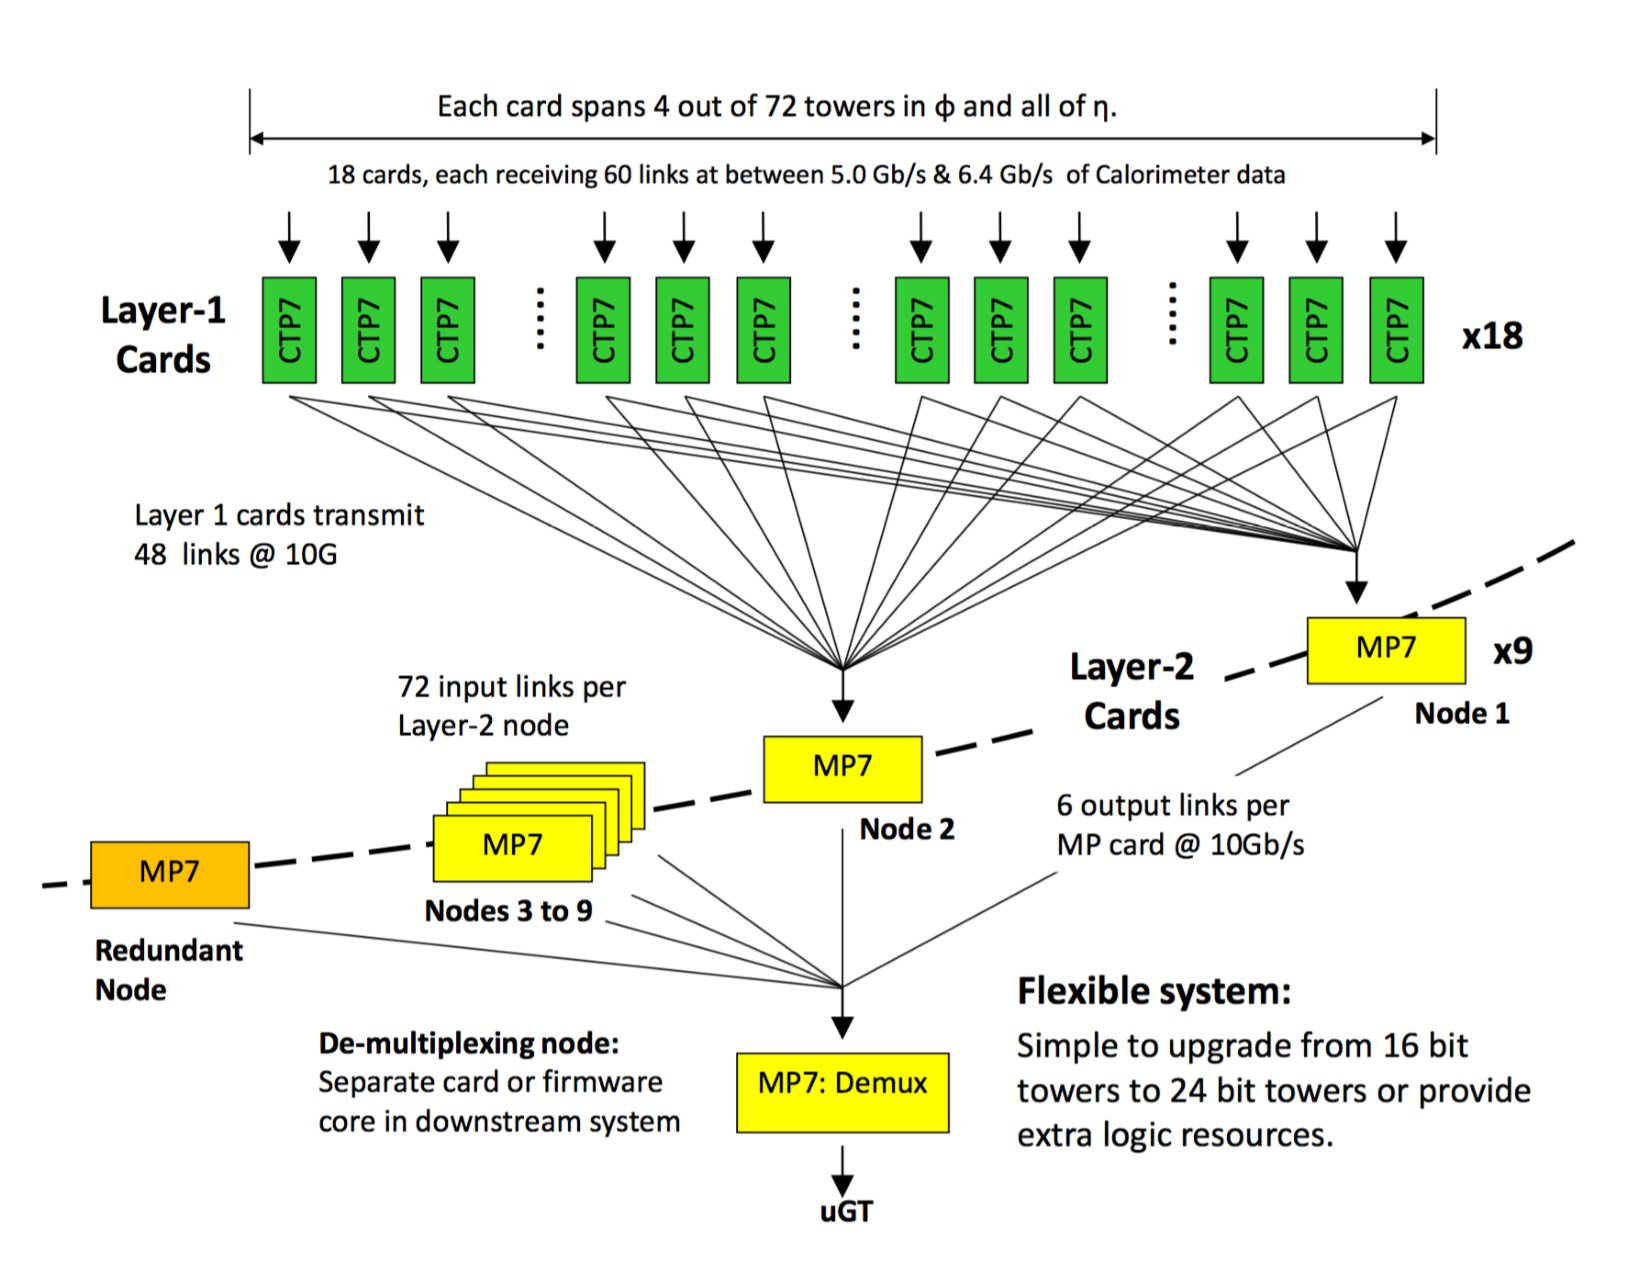
\includegraphics[width=0.49\textwidth]{cms_and_lhc/plots/cms_l1t_hardware.pdf}
     \caption{
(left) System flow chart of the L1 trigger, showing the complete trigger system, and
input detector subsystems.
(right) The L1 calorimeter trigger showing the number of cards and links between
each system.
     }
     \label{fig:cms_l1t}
\end{figure*}

The Calorimeter Layer-1 Trigger systems was designed and built by the University of
Wisconsin--Madison and is currently operated by a team of engineers, research
scientists, and graduate students. I was part of the team of graduate students maintaining
the system and would regularly be on-call in case of any trigger related problems. The
excellent design and engineering that built the Layer-1 CTP7 hardware and firmware
has resulted in a very robust system. More often than not, the Layer-1 on-call
helps other detector systems diagnose their detector and link related problems.



\subsubsection{HLT}
Events which pass the L1 Trigger progress to the HLT. The significantly reduced
event rate, from 40 MHz to 100 kHz, allows for a higher latency trigger which
has access to information from all detector subsystems at full granularity.
Specifically, the full HLT has access to the full ECAL crystal granularity and
information from the inner tracker subsystem. At the start of Run 2, the HLT
was composed of 15,000 commercially available CPU cores running Scientific
Linux~\cite{cms_daq_7097437}. The HLT reconstructs events in a similar way
to what is used offline for events which are already stored. The exception
is that the HLT version is optimized to run quicker with some small sacrifices 
in precision which are mostly related to the track reconstruction 
algorithms~\cite{Khachatryan:2016bia}.

The HLT event processing is centered around the concept of an \texttt{HLT path}.
An \texttt{HLT path} is a sequence of algorithmic processing steps containing
steps which reconstruct physics objects and their attributes and other steps
which make selections filtering out objects which fail certain 
requirements~\cite{Khachatryan:2016bia}. Well constructed HLT paths will
save the most CPU-intensive steps for downstream in the path after many of the
events have been filtered away by failing earlier selections. A good example
of an \texttt{HLT path} which progresses from simple towards more complex and CPU-
intensive is that used for hadronically decaying $\tau$ ($\tauh$) lepton reconstruction.
A common approach to separate $\tauh$ from quark and gluon induced ``jets'' is
to select well-isolated objects; the HLT relies on this exact approach.
The first step of $\tauh$ paths reconstruct basic ``jet''~\ref{sec:obj_reco_jet} objects from
calorimeter information only. Events which reconstruct calorimeter based ``jets''
passing selection criteria move to the next sequence which adds track information 
from the inner tracker to calculate the isolation of the associated ``jet''.
Only after ``jets'' are determined to be well-isolated is the full HLT event 
reconstruction run~\cite{Khachatryan:2016bia}. This reduces computing time significantly
and keeps the $\tauh$ paths within the roughly 200 ms time requirement for
the HLT.

Just like the L1 Trigger, the HLT is used to decide if an event should progress
to the next stage of data processing. In this case, an event which \textit{passes}
an \texttt{HLT path} is saved for future data processing. Events which \textit{fail}
all \texttt{HLT paths} are not stored. The final output rate of the HLT is
about 1000 Hz on average over the full length of a run~\cite{cms_daq_7097437}.



\subsubsection{Tau HLT Upgrades in 2018}
In 2017 and 2018, I have worked to help improve the $\tauh$ \texttt{HLT paths} 
used at CMS. For all previous years, the $\tauh$ \texttt{HLT paths} have used
a cone-based $\tauh$ reconstruction. The cone-based reconstruction 
uses a signal cone of $\dr = 0.18$ containing the $\tau$ lepton decay products,
and has an isolation annulus of $0.18 < \dr < 0.45$. Improvements in the
algorithm are designed to increase the alignment between the offline $\tauh$
reconstruction algorithm and the HLT algorithm. Offline reconstruction uses
the Hadron Plus Strips (HPS) algorithm, see Section~\ref{sec:obj_reco_tau}.
I have transferred the offline HPS algorithm to the HLT and tested its
performance against the previous cone-based reconstruction. For a similar
selection efficiency the HPS algorithm is able to achieve a HLT rate
reduction of roughly 20\%~\ref{fig:hlt_hps}. The HPS \texttt{HLT paths}
will be tested during initial 2018 data taking. If online performance
follow expectations, all of the primary $\tauh$ \texttt{HLT paths}
will be updated to using the HPS algorithm.

\begin{figure*}[htbp]
\centering
     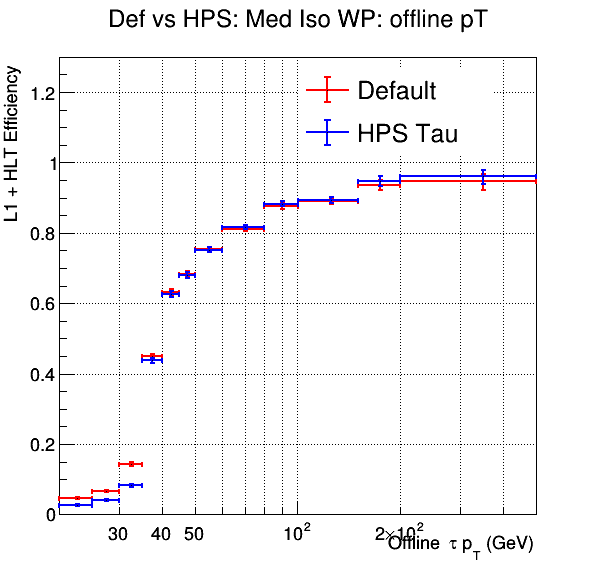
\includegraphics[width=0.55\textwidth]{cms_and_lhc/plots/eff_Def_vs_HPS_Med_Iso_WP_offline_pT.png}
     \caption{
Monte-carlo based efficiency distribution showing the cone-based HLT
algorithm as ``Default'' in red and the HPS-based HLT algorithm
in blue. For nearly identical efficiency performance it is expected that
the HLT rate can be reduced by up to 20\%. FIXME Hopefully I can put in
a plot comparing data efficiency in early 2018, I'm not sure if there
will be time.
     }
     \label{fig:hlt_hps}
\end{figure*}


